% racah — theory note
% Build:  pdflatex theory.tex  (twice, for the table of contents)
% No external packages beyond a standard TeX Live installation; no bibtex.
\documentclass[11pt,a4paper]{article}

\usepackage[margin=1in]{geometry}
\usepackage[T1]{fontenc}
\usepackage[utf8]{inputenc}
\usepackage{lmodern}
\usepackage{microtype}
\usepackage{amsmath,amssymb,amsthm,mathtools}
\usepackage{booktabs}
\usepackage{enumitem}
\usepackage{tcolorbox}
\usepackage{tikz}
\usetikzlibrary{calc}
\usepackage[colorlinks=true,linkcolor=blue,urlcolor=blue,citecolor=blue]{hyperref}

\theoremstyle{plain}
\newtheorem{theorem}{Theorem}[section]
\newtheorem{proposition}[theorem]{Proposition}
\theoremstyle{definition}
\newtheorem{fact}[theorem]{Fact}
\newtheorem{definition}[theorem]{Definition}
\newtheorem{convention}[theorem]{Convention}
\newtheorem{remark}[theorem]{Remark}

% --- Shared TikZ vocabulary: Dynkin diagrams (Sec. 3) and fusion trees
%     (Secs. 11-13). One visual language, no per-diagram tuning. ---
\tikzset{
  diagram/.style={line width=0.55pt, baseline={(0,-0.08)}},
  dnode/.style={circle, draw, fill=white, inner sep=0pt, minimum size=6.5pt},
  dlabel/.style={font=\scriptsize, label distance=2pt},
  fvertex/.style={circle, fill, inner sep=0pt, minimum size=2.4pt},
  fleg/.style={font=\small, inner sep=2pt},
}
% Dynkin diagrams: bonds are drawn first, the white-filled nodes go on top.
% Node: \dnode[label position]{x,y}{Bourbaki index}
\newcommand{\dnode}[3][below]{\node[dnode, label={[dlabel]#1:{$#3$}}] at (#2) {};}
% Single bond, and the dotted elision of a generic-rank chain
\newcommand{\dbond}[2]{\draw (#1) -- (#2);}
\newcommand{\ddotted}[2]{\draw[dotted, line width=0.8pt, shorten <=4pt,
  shorten >=4pt] (#1) -- (#2);}
% Inequality-sign arrow at the midpoint of #1--#2, pointing toward #2
\newcommand{\darrow}[2]{%
  \coordinate (dyc) at ($(#1)!0.5!(#2)$);
  \draw ($($(dyc)!3.5pt!(#1)$)+(0,4pt)$) -- ($(dyc)!4pt!(#2)$)
     -- ($($(dyc)!3.5pt!(#1)$)+(0,-4pt)$);}
% Double / triple bond; the arrow points toward #2 = the SHORT root
\newcommand{\dbondD}[2]{\draw[double, double distance=2.5pt] (#1) -- (#2);%
  \darrow{#1}{#2}}
\newcommand{\dbondT}[2]{\draw[double, double distance=4.2pt] (#1) -- (#2);%
  \draw (#1) -- (#2);\darrow{#1}{#2}}
% Fusion trees: a trivalent splitting vertex (dot) with a multiplicity label
\newcommand{\fvert}[2]{\node[fvertex] at (#1) {};%
  \node[fleg, right=1pt] at (#1) {$#2$};}

\newcommand{\g}{\mathfrak{g}}
\newcommand{\su}{\mathfrak{su}}
\newcommand{\so}{\mathfrak{so}}
\newcommand{\symp}{\mathfrak{sp}}
\newcommand{\Irr}{\mathrm{Irr}}
\newcommand{\Hom}{\mathrm{Hom}}
\newcommand{\End}{\mathrm{End}}
\newcommand{\id}{\mathbb{1}}
\newcommand{\ZZ}{\mathbb{Z}}
\newcommand{\CC}{\mathbb{C}}
\newcommand{\RR}{\mathbb{R}}
\newcommand{\dual}[1]{\bar{#1}}
\newcommand{\code}[1]{\texttt{#1}}
\newcommand{\gaugemd}{\href{https://github.com/Ryo-wtnb11/racah/blob/main/docs/gauge.md}{\code{docs/gauge.md}}}
\newcommand{\gaugeson}{\href{https://github.com/Ryo-wtnb11/racah/blob/main/docs/gauge_soN.md}{\code{docs/gauge\_soN.md}}}
\newcommand{\refsmd}{\href{https://github.com/Ryo-wtnb11/racah/blob/main/docs/references.md}{\code{docs/references.md}}}

\title{\textbf{The representation theory \code{racah} computes}\\[0.3em]
\large A self-contained note built on the Killing--Cartan classification:\\
groups and global forms, irreps, Clebsch--Gordan coefficients,\\
recoupling, and gauge}
\author{The \code{racah} project \\ \small\url{https://github.com/Ryo-wtnb11/racah}}
\date{}

\begin{document}
\maketitle
\thispagestyle{plain}

\begin{tcolorbox}[colback=yellow!8!white,colframe=orange!70!black,
  title=\textbf{Notice: AI-generated document}]
This note was written by an AI agent as reference material for AI agents (and
humans) working on the \code{racah} repository. \textbf{It may contain errors.}
Check every statement against the code and the tests rather than trusting it
blindly.

\medskip
This note is \emph{not} normative. It explains what the objects are and
summarises the prior results the implementation rests on. The \textbf{frozen
normative authority} for every basis, phase, ordering and normalisation
convention --- the actual numeric gauge --- is \gaugemd{} (base $SU(2)$ and
$SU(N)$) and \gaugeson{} ($SO(N)$/$Sp(2N)$), verified by the golden tests.
Where this note and those documents appear to disagree, those documents win.
This note deliberately does not restate their numeric values.
\end{tcolorbox}

\begin{abstract}
\noindent
\code{racah} computes the coefficient data of the fusion category of
finite-dimensional unitary representations of a connected compact simple Lie
group. The note starts from the Killing--Cartan classification of the simple
Lie algebras --- $A_r$, $B_r$, $C_r$, $D_r$, $G_2$, $F_4$, $E_6$, $E_7$, $E_8$
--- derives the compact groups and their global forms from it, and then defines
the coefficients: irrep labels and dimensions, dualities and Frobenius--Schur
indicators,
fusion multiplicities, Clebsch--Gordan coefficients, and the recoupling
($F$) and braiding ($R$) symbols, for $SU(2)$, $SU(N)$, $Spin(N)/SO(N)$,
$Sp(2N)$ and their central quotients. This note defines each of those objects,
states the established results from the literature that the implementation
uses, and records --- as equations --- the conventions the crate fixes where the
mathematics leaves a choice. Scope is exactly what the implementation uses; it
is not a course in Lie theory.
\end{abstract}

\tableofcontents
\bigskip

%======================================================================
\section{Scope, and how to read this note}
%======================================================================

\code{racah} is a coefficient library. Its outputs are numbers attached to
tuples of irrep labels, and every one of those numbers is only defined
\emph{relative to a choice of basis}. The note is therefore organised around
three questions, in order:

\begin{enumerate}[label=(\roman*),leftmargin=2.2em]
  \item \textbf{What is the object?} A definition, with every symbol defined
    before use (Sections~\ref{sec:classification}--\ref{sec:pentagon}).
  \item \textbf{What does the literature already establish about it?} The
    prior results the implementation depends on, stated as facts with
    attribution. These are gathered in the section where they are used and
    flagged as \textbf{Fact}.
  \item \textbf{What does \code{racah} choose?} Where the mathematics leaves a
    free choice, the choice is stated here as an equation or a rule, and the
    normative document holding the frozen values is named.
\end{enumerate}

\paragraph{The classification is the spine.} The note is built on the
Killing--Cartan classification, not on a list of groups. Section~\ref{sec:classification}
states the classification and draws the nine Dynkin diagrams;
Section~\ref{sec:global} turns each family into a compact simply connected
group with a known centre, and each subgroup of that centre into a global
form; Section~\ref{sec:racah} then says which entries of the classification
\code{racah} actually computes for and by which code path. Everything after
that --- highest weights, bases, fusion, CGC, $F$ and $R$ --- refers back to
those three sections rather than re-deriving where the families come from.
This mirrors the crate: \code{group::RootSystem} carries all nine families and
\code{group::GroupId} is a root system paired with a global form.

\paragraph{Two constructions, two normative documents.} The crate has three
coefficient engines but only two constructions. $SU(2)$ is evaluated from
closed forms; $SU(N)$ is built on the Gelfand--Tsetlin basis; $SO(N)$ and
$Sp(2N)$ are built by a generator bootstrap. Section~\ref{sec:constructions}
explains why the branching structure of each family forces the choice.

\paragraph{Citation numbering.} Numbered citations $[n]$ in this note use the
\emph{same numbering} as \refsmd{}, which additionally carries the
\code{file:symbol}-level port provenance. Entries $[1]$--$[13]$ are that
document's bibliography verbatim; $[14]$--$[21]$ are added here for results
this note states that \refsmd{} did not previously need to source. Every
\textbf{Fact} and every mathematical table row carries a numbered citation
with section-level precision; the tables of Section~\ref{sec:racah} are the
one exception, and cite this repository's own normative documents and tests
instead, because they state facts about the crate rather than about
mathematics.

%======================================================================
\section{Notation}
%======================================================================

\noindent
\begin{tabular}{@{}ll@{}}
\toprule
Symbol & Meaning \\
\midrule
$G$ & a connected compact Lie group with simple Lie algebra \\
$\g$, $r$ & its Lie algebra (complexified where convenient), and the rank of $\g$ \\
$\mathfrak{h}$, $\mathfrak{h}^*$ & a Cartan subalgebra and its dual (where weights live) \\
$\Phi$, $\Phi^+$, $\Delta$ & the roots, the positive roots, the simple roots $\alpha_1,\dots,\alpha_r$ \\
$\alpha^\vee = 2\alpha/(\alpha,\alpha)$ & the coroot of $\alpha$ \\
$\rho = \tfrac12\sum_{\alpha\in\Phi^+}\alpha$ & the Weyl vector \\
$P$, $Q$, $P^+$ & the weight lattice, the root lattice, the dominant integral weights \\
$W$ & the Weyl group \\
$\varepsilon_1,\dots,\varepsilon_n$ & the orthonormal ($\varepsilon$) basis of $\mathfrak{h}^*$ used by the combinatorics \\
$\lambda$ & a highest weight; $\lambda_i = (\lambda,\varepsilon_i)$ its $\varepsilon$-components \\
$a_i = \langle\lambda,\alpha_i^\vee\rangle$ & the $i$-th Dynkin label of $\lambda$ (Bourbaki numbering $[20]$) \\
$a,b,c,d,e,f$ & irreps of $G$, identified with their highest weights \\
$V_a$, $d_a=\dim V_a$ & the carrier space of $a$ and its dimension \\
$\dual a$ & the dual (complex-conjugate) irrep of $a$ \\
$\mathbf{1}$ & the trivial irrep \\
$m_a$ & a basis (``magnetic'') index inside $V_a$, $1\le m_a\le d_a$ \\
$N^c_{ab}$ & the fusion multiplicity: how many copies of $c$ occur in $a\otimes b$ \\
$\mu,\nu,\kappa,\lambda$ & outer-multiplicity indices; these are the four $F$-block multiplicity axes\footnotemark \\
$C^{c\mu}_{a\,m_a;\,b\,m_b}$ & a Clebsch--Gordan coefficient for the channel $(a,b\to c,\mu)$ \\
$P^c_{ab}$ & the orthogonal projector onto the $c$-isotypic component of $V_a\otimes V_b$ \\
$[F^{abc}_d]_{(e,\mu\nu),(f,\kappa\lambda)}$ & the $F$-symbol (associator) for fusing $a,b,c$ into $d$ \\
$[R^{ab}_c]_{\mu\nu}$ & the $R$-symbol (braiding) exchanging $a$ and $b$ inside $c$ \\
$\varkappa_a\in\{+1,-1,0\}$ & the Frobenius--Schur indicator of $a$ \\
$Z(G)$, $\Gamma$ & the centre of $G$, and a subgroup of it that is quotiented out \\
\bottomrule
\end{tabular}

\footnotetext{The name $\lambda$ is overloaded: it is a highest weight
everywhere except on the $F$/$R$ multiplicity axes, where it is the fourth
multiplicity index. Context disambiguates, and $[\mu,\nu,\kappa,\lambda]$ is
what the API calls those axes.}

\medskip
Inner products $(\cdot,\cdot)$ on $\mathfrak{h}^*$ are the ones induced by the
Killing form; $\langle\lambda,\alpha^\vee\rangle = 2(\lambda,\alpha)/(\alpha,\alpha)$.
Overlines denote complex conjugation, daggers Hermitian adjoints.

%======================================================================
\section{The classification of the simple Lie algebras}
\label{sec:classification}
%======================================================================

Every group \code{racah} computes for is a compact form of one entry in a
finite classification, and the crate's type system is a transcription of that
classification: \code{racah::group::RootSystem} has exactly nine variants,
one per family. This section states the classification, draws its diagrams in
the numbering the API uses, and records the rank conventions that make the
list irredundant. It is the backbone the rest of the note hangs off.

\subsection{Root systems, Cartan matrices, Dynkin diagrams}

Let $\g$ be a finite-dimensional complex Lie algebra. It is \emph{simple} if
it is non-abelian and has no proper non-zero ideal, and \emph{semisimple} if
it is a direct sum of simple ideals. Fix a Cartan subalgebra
$\mathfrak{h}\subset\g$ (a maximal self-normalising abelian subalgebra of
semisimple elements); its dimension is the \emph{rank} $r$. The adjoint action
of $\mathfrak{h}$ decomposes $\g$ into root spaces, giving the root system
$\Phi\subset\mathfrak{h}^*$, and a choice of positive system fixes the simple
roots $\Delta=\{\alpha_1,\dots,\alpha_r\}$ (Notation, Section~2). The
\emph{Cartan matrix} is
\begin{equation}\label{eq:cartan}
  A_{ij} \;=\; \langle \alpha_j, \alpha_i^\vee\rangle
        \;=\; \frac{2(\alpha_i,\alpha_j)}{(\alpha_i,\alpha_i)}
        \;\in\;\ZZ,
  \qquad A_{ii}=2,\quad A_{ij}\le 0 \ (i\neq j).
\end{equation}
The \emph{Dynkin diagram} of $\g$ is the graph on $r$ nodes with
$A_{ij}A_{ji}\in\{0,1,2,3\}$ edges between nodes $i\neq j$, decorated --- when
the two roots have different lengths --- with an arrow pointing from the long
root towards the short one. The diagram determines $A$, $A$ determines $\g$
up to isomorphism, and $\g$ is simple exactly when its diagram is connected
(Humphreys $[8]$ \S11.1--\S11.2 for the Cartan matrix and the diagram,
\S14.2 for the isomorphism theorem; Bourbaki $[20]$ Ch.~VI \S1.5, \S4.1).

\begin{theorem}[Killing--Cartan classification]\label{thm:kc}
A complex simple Lie algebra is isomorphic to exactly one of
\[
  A_r\ (r\ge 1),\quad B_r\ (r\ge 2),\quad C_r\ (r\ge 3),\quad D_r\ (r\ge 4),
  \quad G_2,\quad F_4,\quad E_6,\quad E_7,\quad E_8,
\]
with the Dynkin diagrams of Section~\ref{sec:diagrams}. Equivalently: the
connected Dynkin diagrams are exactly those nine shapes. Humphreys $[8]$
\S11.4 (Theorem) with the proof of \S11.4--\S11.5 and the existence
half in \S12.1; Bourbaki $[20]$ Ch.~VI \S4.2 (Theorem~3) and Plates I--IX;
Fulton--Harris $[7]$ \S21.1.
\end{theorem}

The first four are the \emph{classical} families --- they are the ones with a
uniform matrix description, and the only ones \code{racah} computes
coefficients for --- and the last five are the \emph{exceptional} algebras.

\subsection{The nine diagrams, in Bourbaki numbering}
\label{sec:diagrams}

Nodes are drawn $\circ$ and labelled underneath with their Bourbaki index; the
index order is exactly the order of the Dynkin label tuple $(a_1,\dots,a_r)$
that the API accepts and returns (Convention~\ref{conv:labelling}). A double
or triple bond carries an arrow pointing at the \emph{short} root.

\medskip
\noindent
\begin{tabular}{@{}l@{\hspace{2em}}l@{}}
$A_r$, $r\ge 1$ &
  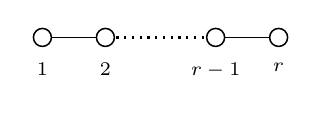
\begin{tikzpicture}[diagram]
    \dbond{0,0}{0.8,0}\ddotted{0.8,0}{2.2,0}\dbond{2.2,0}{3.0,0}
    \dnode{0,0}{1}\dnode{0.8,0}{2}\dnode{2.2,0}{r-1}\dnode{3.0,0}{r}
  \end{tikzpicture} \\[1.6em]
$B_r$, $r\ge 2$ &
  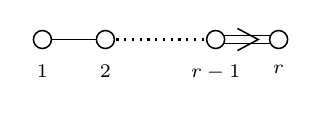
\begin{tikzpicture}[diagram]
    \dbond{0,0}{0.8,0}\ddotted{0.8,0}{2.2,0}\dbondD{2.2,0}{3.0,0}
    \dnode{0,0}{1}\dnode{0.8,0}{2}\dnode{2.2,0}{r-1}\dnode{3.0,0}{r}
  \end{tikzpicture} \\[1.6em]
$C_r$, $r\ge 3$ &
  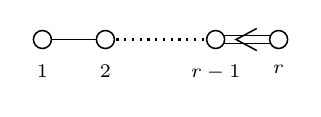
\begin{tikzpicture}[diagram]
    \dbond{0,0}{0.8,0}\ddotted{0.8,0}{2.2,0}\dbondD{3.0,0}{2.2,0}
    \dnode{0,0}{1}\dnode{0.8,0}{2}\dnode{2.2,0}{r-1}\dnode{3.0,0}{r}
  \end{tikzpicture} \\[1.6em]
$G_2$ &
  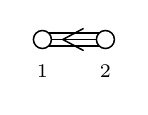
\begin{tikzpicture}[diagram]
    \dbondT{0.8,0}{0,0}
    \dnode{0,0}{1}\dnode{0.8,0}{2}
  \end{tikzpicture} \\[1.6em]
$F_4$ &
  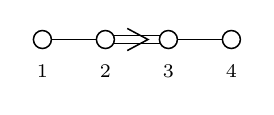
\begin{tikzpicture}[diagram]
    \dbond{0,0}{0.8,0}\dbondD{0.8,0}{1.6,0}\dbond{1.6,0}{2.4,0}
    \dnode{0,0}{1}\dnode{0.8,0}{2}\dnode{1.6,0}{3}\dnode{2.4,0}{4}
  \end{tikzpicture} \\
\end{tabular}

\medskip
\noindent
$D_r$, $r\ge 4$ --- a chain of $r-2$ nodes forking into two:
\begin{center}
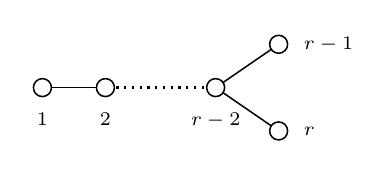
\begin{tikzpicture}[diagram]
  \dbond{0,0}{0.8,0}\ddotted{0.8,0}{2.2,0}
  \dbond{2.2,0}{3.0,0.55}\dbond{2.2,0}{3.0,-0.55}
  \dnode{0,0}{1}\dnode{0.8,0}{2}\dnode{2.2,0}{r-2}
  \dnode[right]{3.0,0.55}{r-1}\dnode[right]{3.0,-0.55}{r}
\end{tikzpicture}
\end{center}

\noindent
$E_8$ --- a chain of seven nodes with node $2$ attached to node $4$:
\begin{center}
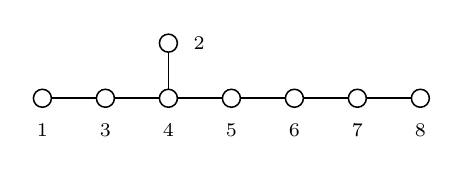
\begin{tikzpicture}[diagram]
  \dbond{0,0}{4.8,0}\dbond{1.6,0}{1.6,0.7}
  \dnode{0,0}{1}\dnode{0.8,0}{3}\dnode{1.6,0}{4}\dnode{2.4,0}{5}
  \dnode{3.2,0}{6}\dnode{4.0,0}{7}\dnode{4.8,0}{8}
  \dnode[right]{1.6,0.7}{2}
\end{tikzpicture}
\end{center}
$E_7$ is the subdiagram on nodes $\{1,\dots,7\}$ and $E_6$ the subdiagram on
$\{1,\dots,6\}$ --- deleting node $8$, then node $7$, from the tail of the
chain (Bourbaki $[20]$ Plates V--VII):
\begin{center}
\begin{tabular}{@{}l@{\hspace{2em}}l@{}}
$E_7$ &
  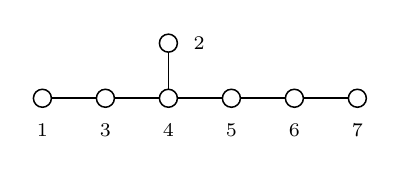
\begin{tikzpicture}[diagram]
    \dbond{0,0}{4.0,0}\dbond{1.6,0}{1.6,0.7}
    \dnode{0,0}{1}\dnode{0.8,0}{3}\dnode{1.6,0}{4}\dnode{2.4,0}{5}
    \dnode{3.2,0}{6}\dnode{4.0,0}{7}
    \dnode[right]{1.6,0.7}{2}
  \end{tikzpicture} \\[2.2em]
$E_6$ &
  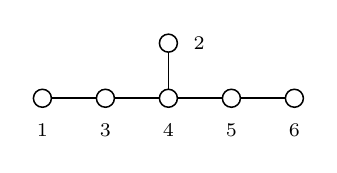
\begin{tikzpicture}[diagram]
    \dbond{0,0}{3.2,0}\dbond{1.6,0}{1.6,0.7}
    \dnode{0,0}{1}\dnode{0.8,0}{3}\dnode{1.6,0}{4}\dnode{2.4,0}{5}
    \dnode{3.2,0}{6}
    \dnode[right]{1.6,0.7}{2}
  \end{tikzpicture} \\
\end{tabular}
\end{center}

\subsection{Why the rank conventions start where they do}
\label{sec:coincidences}

The rank bounds in Theorem~\ref{thm:kc} are not arbitrary: at low rank the
diagram shapes coincide, and without the bounds the list would repeat itself.
The coincidences are exactly

\begin{center}
\begin{tabular}{@{}lll@{}}
\toprule
Diagram coincidence & Algebra isomorphism & Group statement \\
\midrule
$A_1 = B_1 = C_1$ & $\su(2)\cong\so(3)\cong\symp(2)$ & $SU(2)\cong Spin(3)\cong Sp(2)$ \\
$B_2 = C_2$ & $\so(5)\cong\symp(4)$ & $Spin(5)\cong Sp(4)$ \\
$D_2 = A_1\times A_1$ & $\so(4)\cong\su(2)\oplus\su(2)$ & $Spin(4)\cong SU(2)\times SU(2)$ \\
$D_3 = A_3$ & $\so(6)\cong\su(4)$ & $Spin(6)\cong SU(4)$ \\
\bottomrule
\end{tabular}
\end{center}

\noindent
$D_2$ is the only one of the four that is not simple at all: its diagram is
disconnected, so $\so(4)$ is semisimple but not simple, and the theorem does
not apply to it. Each line is a diagram identity first --- read off the shapes
above at $r=1,2,3$ --- and the algebra and group statements follow from
Theorem~\ref{thm:kc} and Fact~\ref{fact:compactform}. Bourbaki $[20]$
Ch.~VI \S4.4 and the Plates I--IV remarks (the identifications of low-rank
systems); Fulton--Harris $[7]$ \S18 (the classical algebras, where the same
isomorphisms are exhibited on the defining representations).

\begin{remark}[What the code does with the coincidences]
\label{rem:lowrank}
\code{racah} takes the coincidences seriously in the $B/C/D$ bootstrap but
does \emph{not} adopt Bourbaki's irredundant bounds verbatim, because a
constructor is named after a \emph{group}, not a diagram. The bootstrap family
key \code{bcd::Series} enforces $r\ge 2$ for $B$ and $C$ and $r\ge 3$ for $D$:
the genuinely duplicated low ranks $B_1$, $C_1$, $D_2$ are rejected with a
per-global-form redirect ($Spin(3)\cong SU(2)$, $Sp(2)\cong SU(2)$,
$Spin(4)\cong SU(2)\times SU(2)$, and for the quotients $SO(3)$/$PSp(2)$ =
integer $j$ only, $SO(4)$ = $j_1+j_2$ integer), while $C_2$ and $D_3$ are
\emph{kept} --- $Sp(4)$ and $SO(6)$ are groups a caller legitimately asks for
by name, and the bootstrap builds them directly rather than routing the caller
through $Spin(5)$ or $SU(4)$. Nothing downstream depends on the redundancy
being removed: the two presentations of the same group give the same
coefficients up to the relabelling, and only the label conventions differ.
API: \code{bcd::Series::min\_rank}, \code{bcd::Series::low\_rank\_redirect}.
\end{remark}

\begin{remark}[Rank versus matrix dimension]
Two integers are in play and they are not the same. $r$ is the rank --- the
number of Dynkin labels. $N$ is the matrix dimension of the defining
representation. The \code{GroupId} constructors take $N$
(\code{GroupId::so(7)}, \code{GroupId::sp(6)}) and convert:
$SU(N)\leftrightarrow A_{N-1}$, $Spin(2r+1)\leftrightarrow B_r$,
$Sp(2r)\leftrightarrow C_r$, $Spin(2r)\leftrightarrow D_r$. Weight tuples are
always indexed by $r$.
\end{remark}

%======================================================================
\section{From algebras to compact groups, and to global forms}
\label{sec:global}
%======================================================================

Theorem~\ref{thm:kc} classifies complex \emph{algebras}. \code{racah} computes
for \emph{compact groups}, and the passage from one to the other is two steps,
neither of them unique in the naive sense: first a compact real form and its
simply connected cover, then a quotient by a subgroup of the centre.

\subsection{Step one: the compact simply connected group}
\label{sec:compactforms}

\begin{fact}[Compact real forms and their covers]\label{fact:compactform}
Every complex simple Lie algebra $\g$ has a compact real form
$\mathfrak{k}\subset\g$, unique up to conjugation, and there is a unique
connected simply connected compact Lie group $G_{\mathrm{sc}}$ with Lie algebra
$\mathfrak{k}$. Its centre is finite, and
\begin{equation}\label{eq:centre}
  Z(G_{\mathrm{sc}}) \;\cong\; P/Q ,
\end{equation}
the weight lattice modulo the root lattice --- a finite abelian group read
straight off the Cartan matrix \eqref{eq:cartan}, since $Q$ is spanned by the
simple roots and $P$ by the fundamental weights. Existence and
conjugacy-uniqueness of the compact real form: Knapp $[21]$ Theorem~6.11 and
Corollary~6.20. The centre: Br\"ocker--tom Dieck $[14]$ \S V.7;
Humphreys $[8]$ \S13.1 for the $P/Q$ computation itself.
\end{fact}

Applying \eqref{eq:centre} family by family gives the table this note and the
crate both rest on. It is the dictionary between the classification and the
group names in the API.

\begin{center}
\small
\begin{tabular}{@{}llll@{}}
\toprule
Family & Compact simply connected $G_{\mathrm{sc}}$ & $Z(G_{\mathrm{sc}})\cong P/Q$ & Adjoint form $G_{\mathrm{sc}}/Z$ \\
\midrule
$A_{N-1}$, $N\ge 2$ & $SU(N)$      & $\ZZ_N$ & $PSU(N)$ \\
$B_r$, $r\ge 2$     & $Spin(2r+1)$ & $\ZZ_2$ & $SO(2r+1)=PSO(2r+1)$ \\
$C_r$, $r\ge 2$     & $Sp(2r)$     & $\ZZ_2$ & $PSp(2r)$ \\
$D_r$, $r$ odd      & $Spin(2r)$   & $\ZZ_4$ & $PSO(2r)$ \\
$D_r$, $r$ even     & $Spin(2r)$   & $\ZZ_2\times\ZZ_2$ & $PSO(2r)$ \\
$G_2$               & $G_2$        & $1$     & $G_2$ \\
$F_4$               & $F_4$        & $1$     & $F_4$ \\
$E_6$               & $E_6$        & $\ZZ_3$ & $E_6/\ZZ_3$ \\
$E_7$               & $E_7$        & $\ZZ_2$ & $E_7/\ZZ_2$ \\
$E_8$               & $E_8$        & $1$     & $E_8$ \\
\bottomrule
\end{tabular}
\end{center}

\noindent
\emph{Sources for the table.} Each $P/Q$ is tabulated system by system in
Bourbaki $[20]$ Plates I--IX (the plate for each family lists $P/Q$ and the
fundamental weights); the identification with $Z(G_{\mathrm{sc}})$ is
Fact~\ref{fact:compactform}. The $D_r$ split is the arithmetic of the plate
for $D_r$: $P/Q$ is generated by $[\omega_1]$, $[\omega_{r-1}]$,
$[\omega_r]$ with $2[\omega_r] = [\omega_1]$ when $r$ is odd (so the group is
cyclic of order $4$) and $2[\omega_r]=0$ when $r$ is even (so it is
$\ZZ_2\times\ZZ_2$) --- the parity dependence traces to
$(\omega_r,\omega_r)=r/4$. The congruency classes of every family are also
tabulated by Slansky $[13]$ \S5.

\medskip
\noindent
Three families ($G_2$, $F_4$, $E_8$) have trivial centre, so for them
``simply connected'' and ``adjoint'' name the same group and there is no
global-form question to ask at all. These centres are recorded in the
\code{RootSystem} variant docs and are the reason the exceptional variants
carry no admissibility logic (Section~\ref{sec:racah}).

\subsection{Step two: global forms are centre quotients}

Everything the rest of this note computes is stated for a group, but a root
system names only an algebra. $\so(N)$ is the algebra of both $Spin(N)$ and
$SO(N)=Spin(N)/\ZZ_2$; $\su(N)$ is the algebra of $SU(N)$, of $SU(N)/\ZZ_k$ for
every $k\mid N$, and of $PSU(N)=SU(N)/\ZZ_N$. These groups have the same
Lie-algebra representation theory and differ in exactly one respect: which
dominant integral weights are genuine representations \emph{of the group}.


\begin{fact}[Classification of connected compact forms]\label{fact:forms}
Let $G_{\mathrm{sc}}$ be the simply connected compact group with a given root
system. Then $Z(G_{\mathrm{sc}}) \cong P/Q$, every connected compact group with
that root system is $G_\Gamma = G_{\mathrm{sc}}/\Gamma$ for a subgroup
$\Gamma\subseteq Z(G_{\mathrm{sc}})$, and
\begin{equation}\label{eq:admis}
  \Irr(G_\Gamma)
  \;=\; \bigl\{\, \lambda\in P^+ \;:\; \chi_\lambda\big|_\Gamma = 1 \,\bigr\},
\end{equation}
where the \emph{central character} $\chi_\lambda$ depends on $\lambda$ only
through its class $[\lambda]\in P/Q$. $[7]$ \S23; the congruency classes are
tabulated by Slansky $[13]$ \S5.
\end{fact}

The class $[\lambda]\in P/Q$ is the \emph{$N$-ality} / congruency class, and
for the series \code{racah} implements it is an explicit linear form in the
Dynkin labels.

\paragraph{$A_{r}$, $r=N-1$: $P/Q\cong\ZZ_N$.} The class is the $N$-ality
\begin{equation}\label{eq:nality}
  t(\lambda) \;\equiv\; \sum_{i=1}^{N-1} i\,a_i \pmod N ,
\end{equation}
and for $\Gamma = \ZZ_k$ with $k\mid N$ the admissibility condition
\eqref{eq:admis} reads $t(\lambda)\equiv 0 \pmod k$. So $PSU(3)=SU(3)/\ZZ_3$
admits the adjoint $\mathbf{8}$ and rejects the fundamental $\mathbf{3}$.

\paragraph{$B_r$: $P/Q\cong\ZZ_2$.} The class is $a_r \bmod 2$ --- exactly the
tensor/spinor split described in Section~\ref{sec:bcd}. $Spin(2r+1)$ admits all
$\lambda\in P^+$; $SO(2r+1)$ admits those with $a_r$ even.

\paragraph{$C_r$: $P/Q\cong\ZZ_2$.} The class is
$a_1+a_3+a_5+\cdots \bmod 2$. $Sp(2r)$ admits all $\lambda\in P^+$;
$PSp(2r)=Sp(2r)/\ZZ_2$ admits those with $a_1+a_3+\cdots$ even.

\paragraph{$D_r$: $P/Q\cong\ZZ_4$ ($r$ odd) or $\ZZ_2\times\ZZ_2$ ($r$ even).}
This is the rich case, and it is where a convention has to be pinned rather
than derived, because naming a form requires choosing a generator of the
centre.

One condition is uniform in $r$: the \emph{vector} (tensor) sublattice
$\{0,v\}\subset P/Q$ is always a $\ZZ_2$, and quotienting by it gives
\begin{equation}\label{eq:so2r}
  SO(2r):\qquad a_{r-1} + a_r \;\equiv\; 0 \pmod 2 ,
\end{equation}
for every $r$ --- this is the tensor/spinor split described in
Section~\ref{sec:bcd},
and it is $r$-uniform because $(\varepsilon_1,\varepsilon_1)=1$ for every $r$.
The remaining forms depend on the parity of $r$.

For $r$ odd the class is valued in $\ZZ_4$, and \code{racah} fixes the
generator $c=[\omega_r]$, so that
\begin{equation}\label{eq:d4class}
  \kappa(\lambda) \;\equiv\;
    a_r - a_{r-1} + 2\!\!\sum_{\substack{i \ \mathrm{odd} \\ i \le r-2}}\!\! a_i
  \pmod 4 .
\end{equation}
This choice makes conjugation \emph{be} negation of the class, matching
$\code{bcd::Irrep::dual}$ ($\lambda_r\mapsto-\lambda_r$). Slansky's uniform
formula $[13]$ \S5 equals $+\kappa$ for $r\equiv 1 \pmod 4$ and $-\kappa$ for
$r\equiv 3\pmod 4$; the difference is the $\ZZ_4$ automorphism $x\mapsto -x$,
i.e. a generator choice, not a discrepancy.

so \eqref{eq:so2r} is the $\kappa\equiv 0\pmod 2$ subgroup, and $PSO(2r)$ (the
full $\ZZ_4$ quotient) is $\kappa\equiv 0 \pmod 4$. There are no half-spin
forms for $r$ odd: $\ZZ_4$ has only one subgroup of order $2$.

For $r$ even the class is valued in $\ZZ_2\times\ZZ_2$, which has three
subgroups of order $2$, so alongside $Spin(2r)$ (all $\lambda$), $SO(2r)$
\eqref{eq:so2r} and $PSO(2r)$ (the full quotient) there are two
\emph{half-spin} forms. Writing
$t \equiv \sum_{i\ \mathrm{odd},\, i\le r-2} a_i \pmod 2$ and
$p \equiv a_{r-1}+t$, $q \equiv a_r + t \pmod 2$:
\[
  \text{half-spin}_+:\ p \equiv 0;\qquad
  \text{half-spin}_-:\ q \equiv 0;\qquad
  PSO(2r):\ p \equiv q \equiv 0 \pmod 2 .
\]
A half-spin form admits one chirality of spinor but \emph{not} the vector
representation (which has $p=q=1$). The two half-spin forms are named for the
class they \emph{retain}, not the central element they kill: a
kill-based name is not uniform in $r$, because $(\omega_r,\omega_r)=r/4$ makes
the annihilator of $z_{\omega_r}$ differ between $r\equiv0$ and $r\equiv2
\pmod 4$. Slansky's $S_s/S_c$ are accepted as documented aliases. \refsmd{}
carries this convention with its full justification.

\subsection{Two consequences the implementation relies on}

\begin{proposition}[Admissibility is a construction-time predicate]
The class map $P^+\to P/Q$, $\lambda\mapsto[\lambda]$, is the restriction of a
group homomorphism, so $[\lambda+\mu]=[\lambda]+[\mu]$ and
$[-w_0\lambda]=-[\lambda]$. Hence the admissible set of \eqref{eq:admis} is
closed under fusion and under duality: it never needs re-checking on a fusion
output.
\end{proposition}

\begin{proposition}[A global form deletes irreps; it never changes a coefficient]
\label{prop:samecoeff}
Let $\lambda$ be admissible for both $G_\Gamma$ and $G_{\Gamma'}$. The
representations of $G_\Gamma$ and $G_{\Gamma'}$ with highest weight $\lambda$
have the same carrier, the same $\g$-action, and hence the same CGC, $F$, $R$
and $\varkappa$ \emph{in the same basis}: the choice of $\Gamma$ never enters
their computation. Consequently the coefficient caches are keyed on irrep
labels with \emph{no global form in the key}, and two forms sharing an irrep
must share the cache entry.
\end{proposition}

\begin{sloppypar}
API: \code{racah::group} --- \code{RootSystem}, \code{GlobalForm},
\code{CenterSubgroup}, \code{GroupId}, and the predicate
\code{GroupId::admits}; the form-aware constructors
\code{sun::Irrep::from\_dynkin\_in} and \code{bcd::Irrep::from\_dynkin\_in}
(the plain \code{from\_dynkin} constructors keep their historically published
groups).
\end{sloppypar}

\begin{remark}[Scope]
Connected compact groups only. $O(N)$ and $Pin(N)$ are not central quotients of
a simply connected group --- they are disconnected extensions --- and are out
of scope; so is any non-compact real form.
\end{remark}

%======================================================================
\section{What \code{racah} implements, against the classification}
\label{sec:racah}
%======================================================================

Sections~\ref{sec:classification} and~\ref{sec:global} describe every simple
compact group. \code{racah} does not compute for all of them. This section is
the correspondence table --- which entry of the classification is served by
which code path, and what happens at the entries that are not served. It cites
the repository's own normative documents and tests rather than the literature:
these are facts about this crate, not about mathematics.

\begin{center}
\small
\begin{tabular}{@{}p{2.1cm}p{2.5cm}p{3.1cm}p{5.4cm}@{}}
\toprule
Family & Groups & Engine & Where it lives \\
\midrule
$A_1$ & $SU(2)$, $SO(3)$ &
  closed forms (Section~\ref{sec:su2}) &
  \code{su2}; exact $3j$/$6j$; gauge \gaugemd{} \\
$A_{N-1}$ & $SU(N)$, $SU(N)/\ZZ_k$, $PSU(N)$ &
  Gelfand--Tsetlin (Section~\ref{sec:gt}) &
  \code{sun}; gauge \gaugemd{} \\
$B_r$ & $Spin(2r+1)$, $SO(2r+1)$ &
  generator bootstrap (Section~\ref{sec:bcd}) &
  \code{bcd}, \code{Series::B}; gauge \gaugeson{} \\
$C_r$ & $Sp(2r)$, $PSp(2r)$ &
  generator bootstrap &
  \code{bcd}, \code{Series::C}; gauge \gaugeson{} \\
$D_r$ & $Spin(2r)$, $SO(2r)$, $PSO(2r)$, half-spin &
  generator bootstrap &
  \code{bcd}, \code{Series::D}; gauge \gaugeson{} \\
$G_2$, $F_4$, $E_6$, $E_7$, $E_8$ & --- &
  none &
  \code{RootSystem} variants only \\
\bottomrule
\end{tabular}
\end{center}

\paragraph{Two types, two jobs.} \code{RootSystem} is the
\emph{label-lattice} type: it carries all nine families of
Theorem~\ref{thm:kc}, it fixes the rank (hence the length of the Dynkin tuple)
and the lattice $P/Q$ (hence the congruences of
Section~\ref{sec:global}). \code{bcd::Series} is the \emph{bootstrap-family}
key: it exists only where a defining-representation seed and a canonical
catalogue exist, so it has exactly three variants $B$, $C$, $D$. The single
bridge is \code{bcd::Series::root\_system}; neither type is an alias of the
other. $A$-series labels are not a \code{Series} at all --- they go through
\code{sun::Irrep} (and $A_1$ through \code{su2}).

\paragraph{A group is a root system plus a global form.} The whole of
\code{GroupId} is
\begin{align*}
  \code{GroupId} \;&=\; \code{RootSystem} \;\times\; \code{GlobalForm}, \\
  \code{GlobalForm} \;&\in\; \{\,\code{SimplyConnected}\,\}\cup
                        \{\,\code{Quotient}(\Gamma) : \Gamma\subseteq Z\,\},
\end{align*}
which is exactly Fact~\ref{fact:forms}: the classification supplies the first
factor, the centre supplies the second. The named constructors are the
ergonomic surface, and they take the matrix dimension, not the rank
(all are associated functions of \code{GroupId}, and the prefix is dropped in
the table):

\begin{center}
\small
\begin{tabular}{@{}lll@{}}
\toprule
Constructor & Group & Root datum \\
\midrule
\code{su(n)}              & $SU(n)$        & $A_{n-1}$, \code{SimplyConnected} \\
\code{su\_quotient(n,k)}  & $SU(n)/\ZZ_k$, $k\mid n$ & $A_{n-1}$, \code{Zk(k)} \\
\code{psu(n)}             & $PSU(n)$       & $A_{n-1}$, \code{Zk(n)} \\
\code{spin(n)}            & $Spin(n)$      & $B_{(n-1)/2}$ or $D_{n/2}$, \code{SimplyConnected} \\
\code{so(n)}              & $SO(n)$        & $B_{(n-1)/2}$ + \code{Z2}, or $D_{n/2}$ + \code{DVector} \\
\code{pso(n)}             & $PSO(n)$       & $B$ + \code{Z2}; $D_r$ + \code{Z4} ($r$ odd), \code{DFull} ($r$ even) \\
\code{sp(m)}              & $Sp(m)$        & $C_{m/2}$, \code{SimplyConnected} \\
\code{psp(m)}              & $PSp(m)$       & $C_{m/2}$, \code{Z2} \\
\code{half\_spin\_plus(n)}  & $Ss(n)$, $4\mid n$ & $D_{n/2}$, \code{DHalfSpinPlus} \\
\code{half\_spin\_minus(n)} & $Sc(n)$, $4\mid n$ & $D_{n/2}$, \code{DHalfSpinMinus} \\
\bottomrule
\end{tabular}
\end{center}

\begin{sloppypar}
\paragraph{Which form the coefficient engines publish.} A construction engine
works in the \emph{cover} --- the bootstrap needs the spinor seeds, so its
internal catalogue is over $Spin(2r+1)$, $Sp(2r)$, $Spin(2r)$ --- while the
labels a query \emph{publishes} are cut down to a chosen default form:
$SO(2r+1)$ for $B$, $Sp(2r)$ for $C$, $SO(2r)$ for $D$. The form-aware
constructors \code{sun::Irrep::from\_dynkin\_in} and
\code{bcd::Irrep::from\_dynkin\_in} take a \code{GroupId} explicitly; the plain
\code{from\_dynkin} constructors keep those historically published defaults.
API: \code{bcd::Series::cover\_group}, \code{bcd::Series::published\_group}.
\end{sloppypar}

\paragraph{The exceptionals are placeholders, and provably inert.}
$G_2$, $F_4$, $E_6$, $E_7$, $E_8$ exist as \code{RootSystem} variants so that
the type transcribes Theorem~\ref{thm:kc} completely --- rank and centre are
recorded, nothing else. There is no coefficient engine and no congruence
logic: \code{GroupId::admits} answers \code{true} for
\code{SimplyConnected} (the cover admits every dominant integral weight, which
needs no family-specific arithmetic) and \code{false} for \emph{every}
quotient, including the mathematically real ones such as $E_6/\ZZ_3$. That is
not a silent wrong answer but the deliberate fail-closed behaviour of
Section~\ref{sec:global}: a group with no admissible weights has no irreps, so
both form-aware constructors reject every label with the ordinary
not-admissible error. It is pinned by the test
\code{tests/global\_form.rs::nonsensical\_root\_datum\_admits\_nothing}, which
sweeps labels for a list of impossible root data --- $E_6$ with
$\ZZ_3$ among them --- and asserts that nothing is admitted.


%======================================================================
\section{Compact groups and their irreducible representations}
\label{sec:compact}
%======================================================================

Let $G$ be a compact Lie group and $V$ a finite-dimensional complex vector
space. A \emph{representation} is a continuous homomorphism
$\pi: G\to GL(V)$; it is \emph{unitary} if $\pi(g)^\dagger\pi(g)=\id$ for all
$g$, and \emph{irreducible} (an \emph{irrep}) if the only $\pi$-invariant
subspaces of $V$ are $0$ and $V$. Write $\Irr(G)$ for the set of isomorphism
classes of irreps.

The whole subject rests on three classical results, which are what make
``coefficient library'' a well-posed idea at all.

\begin{fact}[Unitarisability and complete reducibility; Weyl]
\label{fact:cr}
Every finite-dimensional representation of a compact group admits an invariant
Hermitian inner product (average any inner product against the Haar measure),
and decomposes as a direct sum of irreps. All irreps are
finite-dimensional. See Br\"ocker--tom Dieck $[14]$ \S II.1--II.4, or
Fulton--Harris $[7]$ \S9.
\end{fact}

Consequently every representation \code{racah} touches may be taken unitary
with an orthonormal basis, and every tensor product decomposes.

\begin{fact}[Schur's lemma]\label{fact:schur}
If $a,b$ are irreps then $\Hom_G(V_a,V_b)$ --- the space of linear maps
commuting with the action --- is $\CC$ if $a\cong b$ and $0$ otherwise. More
generally, for representations $V,W$, $\dim\Hom_G(V,W)$ counts the common
irreducible constituents with multiplicity. $[14]$ \S II.1, $[7]$ \S1.2.
\end{fact}

\begin{fact}[Peter--Weyl and Schur orthogonality]\label{fact:pw}
The matrix coefficients $\sqrt{d_a}\,\pi^a_{mn}$ over all $a\in\Irr(G)$ form an
orthonormal basis of $L^2(G)$ with respect to normalised Haar measure; in
particular
\[
  \int_G \overline{\pi^a_{m n}(g)}\;\pi^b_{m' n'}(g)\,dg
   \;=\; \frac{1}{d_a}\,\delta_{ab}\,\delta_{m m'}\,\delta_{n n'}.
\]
$[14]$ \S III.3, $[7]$ \S9. Schur orthogonality is the source of the
Clebsch--Gordan orthonormality and completeness relations of
Section~\ref{sec:cgc}: those relations are not conventions, they are theorems.
\end{fact}

Restricting attention to $G$ connected with $\g$ simple, $\Irr(G)$ is
classified by highest weights, which is the subject of the next section.

%======================================================================
\section{Highest weights, Dynkin labels, dimensions}
\label{sec:hw}
%======================================================================

Fix a maximal torus $T\subset G$ with Lie algebra $\mathfrak{t}$, and let
$\mathfrak{h} = \mathfrak{t}\otimes\CC$ be the corresponding Cartan subalgebra
of $\g_\CC$. A representation $V$ decomposes into simultaneous eigenspaces of
$\mathfrak{h}$,
\[
  V \;=\; \bigoplus_{\omega\in\mathfrak{h}^*} V_\omega,
  \qquad
  V_\omega = \{\, v\in V : H\cdot v = \omega(H)\,v \ \ \forall H\in\mathfrak{h}\,\},
\]
and the $\omega$ with $V_\omega\neq 0$ are the \emph{weights} of $V$, with
\emph{multiplicity} $\dim V_\omega$. The weights of the adjoint representation
other than $0$ are the \emph{roots} $\Phi$. A choice of positive system
$\Phi^+$ picks out simple roots $\Delta=\{\alpha_1,\dots,\alpha_r\}$; a weight
$\lambda$ is \emph{dominant integral} if
$a_i := \langle\lambda,\alpha_i^\vee\rangle \in \ZZ_{\ge 0}$ for all $i$, and
the tuple $(a_1,\dots,a_r)$ is its vector of \emph{Dynkin labels}.

\begin{fact}[Theorem of the highest weight; Cartan--Weyl]\label{fact:hw}
For $G$ connected compact simply connected with simple $\g$, the map
$V\mapsto$ (its highest weight, in the dominance order induced by $\Phi^+$)
is a bijection $\Irr(G)\to P^+$. Each irrep has a one-dimensional highest
weight space, annihilated by every raising operator $e_{\alpha_i}$.
Humphreys $[8]$ \S20--21; $[7]$ \S14.
\end{fact}

\begin{convention}[Labelling]\label{conv:labelling}
\code{racah} accepts and returns irreps as Dynkin label tuples
$(a_1,\dots,a_r)$ in \textbf{Bourbaki numbering} $[20]$ (so, e.g., for $B_r$
the short simple root is $\alpha_r$ and $a_r$ is the spinor label). Internally
the combinatorics use the $\varepsilon$-basis components
$\lambda=(\lambda_1\ge\lambda_2\ge\cdots)$; the two are related by the
series-specific linear map, and both directions are exact integer (or
half-integer, for spinors) arithmetic. API: \code{sun::Irrep::from\_dynkin},
\code{bcd::Irrep::from\_dynkin}.
\end{convention}

\begin{fact}[Weyl dimension formula]\label{fact:weyldim}
For $\lambda\in P^+$,
\begin{equation}\label{eq:weyldim}
  d_\lambda \;=\; \prod_{\alpha\in\Phi^+}
    \frac{(\lambda+\rho,\,\alpha)}{(\rho,\,\alpha)} .
\end{equation}
$[8]$ \S24.3, $[7]$ \S24.3. The right-hand side is a ratio of integers and is
evaluated exactly.
\end{fact}

\begin{fact}[Freudenthal's recursion]\label{fact:freudenthal}
The weight multiplicities $m_\lambda(\omega)=\dim V_\omega$ of $V_\lambda$
satisfy
\begin{equation}\label{eq:freudenthal}
  \bigl( \|\lambda+\rho\|^2 - \|\omega+\rho\|^2 \bigr)\, m_\lambda(\omega)
  \;=\; 2 \sum_{\alpha\in\Phi^+}\ \sum_{k\ge 1}
        m_\lambda(\omega+k\alpha)\,(\omega+k\alpha,\alpha),
\end{equation}
which determines every $m_\lambda(\omega)$ downward from
$m_\lambda(\lambda)=1$. $[8]$ \S22.3.
\end{fact}

Equations~\eqref{eq:weyldim} and~\eqref{eq:freudenthal} are pure integer
combinatorics; \code{racah} computes both in exact arithmetic, with QSpace
$[3]$ used as the independent numerical dimension oracle for $B/C/D$.

%======================================================================
\section{The families, their bases, and the two constructions}
\label{sec:constructions}
%======================================================================

The coefficients of Sections~\ref{sec:cgc}--\ref{sec:pentagon} are defined only
once an orthonormal basis has been chosen inside every $V_a$. The two
constructions \code{racah} implements are two ways of producing that basis, and
which one a family gets is forced by its branching structure.

\subsection{$A$-series: Gelfand--Tsetlin patterns}
\label{sec:gt}

\begin{fact}[Weyl branching for the unitary chain]\label{fact:branch}
Restricting an irrep of $U(k)$ with highest weight
$\lambda=(\lambda_1\ge\cdots\ge\lambda_k)$ to $U(k-1)$ gives
\[
  V^{U(k)}_\lambda\big|_{U(k-1)} \;=\; \bigoplus_{\mu} V^{U(k-1)}_\mu,
  \qquad
  \lambda_1 \ge \mu_1 \ge \lambda_2 \ge \mu_2 \ge \cdots \ge \mu_{k-1} \ge \lambda_k,
\]
each admissible $\mu$ occurring \emph{exactly once}: the chain is
\emph{multiplicity-free}. $[7]$ \S6.1, \S15.3.
\end{fact}

Iterating $U(N)\supset U(N-1)\supset\cdots\supset U(1)$ therefore labels each
basis vector of an $SU(N)$ irrep uniquely by the whole tower of intermediate
highest weights --- a triangular array
\[
  m \;=\;
  \bigl( m_{k,l} \bigr)_{1\le k\le l\le N},
  \qquad
  m_{k,l+1} \ \ge\ m_{k,l} \ \ge\ m_{k+1,l+1},
\]
the \emph{Gelfand--Tsetlin (GT) pattern}, whose top row $l=N$ is $\lambda$.

\begin{fact}[Gelfand--Tsetlin]\label{fact:gt}
The GT patterns with top row $\lambda$ index an orthonormal basis of
$V_\lambda$, and the generators of $\g\mathfrak{l}_N$ act on it by explicit
closed-form matrix elements: the Cartan generators are diagonal with
\[
  \mathrm{wt}(m)_l \;=\; \mathrm{rowsum}(l) - \mathrm{rowsum}(l-1),
  \qquad \mathrm{rowsum}(l) = \sum_{k=1}^{l} m_{k,l},
\]
and the elementary raising/lowering operators $E_{l,l+1}$, $E_{l+1,l}$ have
matrix elements given by a ratio of products of linear forms in the pattern
entries. Original statement: Gelfand--Tsetlin $[4]$; the explicit matrix
elements and their derivation: Baird--Biedenharn $[15]$; a modern account
covering the classical series: Molev $[12]$.
\end{fact}

The uniqueness of the labelling is what makes the ladder elements closed-form,
and that closed form is what makes a direct, exact CGC construction possible.
Two points are worth stating because they are frequently confused:

\begin{remark}
The $SU$ chain \emph{alone} is not multiplicity-free: the adjoint $\mathbf{8}$
of $SU(3)$ restricts to $SU(2)$ as
$\mathbf{2}\oplus\mathbf{2}\oplus\mathbf{3}\oplus\mathbf{1}$. It is the
intermediate $U(1)$ charge at each step that separates the recurring copies,
which is why the chain is written with $U(k)$, not $SU(k)$.
\end{remark}

\begin{convention}[GT basis order]
The magnetic indices $m_a$ of every $SU(N)$ coefficient are positions in
\code{racah}'s GT enumeration order, which reproduces
SUNRepresentations.jl $[9]$ index-for-index and is pinned by checked-in
fixtures. This order is \emph{load-bearing}: a re-enumeration emitting the same
set of patterns in a different order permutes every returned coefficient. The
normative statement, including which pattern occupies the last basis index, is
\gaugemd{} \S1.
\end{convention}

The construction is then: enumerate GT patterns; build the exact rational
ladder matrices of Fact~\ref{fact:gt}; solve the highest-weight nullspace;
gauge-fix; descend by the lowering operators. This is the algorithm of Alex,
Kalus, Huckleberry and von~Delft $[1]$, whose reference implementation
SUNRepresentations.jl $[9]$ \code{racah} ports. Steps and tolerances:
\gaugemd{} \S2--\S7.

\subsection{$B$, $C$, $D$: weights, spinors, and the generator bootstrap}
\label{sec:bcd}

For the orthogonal and symplectic series the $\varepsilon$-basis description is
the practical one. With $\lambda = \sum_i \lambda_i\varepsilon_i$:

\begin{itemize}[leftmargin=1.4em]
  \item $B_r = \so(2r+1)$: $\lambda_1\ge\cdots\ge\lambda_r\ge 0$, all
    $\lambda_i$ simultaneously integers (\emph{tensor} irreps) or all
    half-odd-integers (\emph{spinor} irreps). The Dynkin label $a_r$ is even in
    the tensor sector, odd in the spinor sector.
  \item $C_r = \symp(2r)$: $\lambda_1\ge\cdots\ge\lambda_r\ge 0$, all integers.
    There is no spinor sector; the $\ZZ_2$ centre is detected by
    $a_1+a_3+a_5+\cdots$.
  \item $D_r = \so(2r)$: $\lambda_1\ge\cdots\ge\lambda_{r-1}\ge|\lambda_r|$,
    with $\lambda_r$ of \emph{either sign} --- the sign distinguishes the two
    chiralities, and swapping it is the outer automorphism exchanging the two
    half-spin fundamentals $\omega_{r-1}$ and $\omega_r$. Again all $\lambda_i$
    integral (tensor) or all half-odd-integral (spinor).
\end{itemize}

Root data, the $\varepsilon\leftrightarrow$ Dynkin maps, and the spinor sectors
are Fulton--Harris $[7]$ \S\S18--20, 24 and Humphreys $[8]$ \S12--13. Low ranks
where the classification degenerates ($B_1$, $C_1$, $D_2$) are rejected and
redirected by the API rather than silently aliased.

\paragraph{Why not GT here.}

\begin{fact}[Branching for the orthogonal and symplectic chains]
\label{fact:bcdbranch}
$SO(n)\supset SO(n-1)$ is multiplicity-free, and explicit GT-type bases with
closed-form matrix elements exist for it $[4,12]$. The symplectic chain
$Sp(2r)\supset Sp(2r-2)$ is \emph{not} multiplicity-free: intermediate irreps
recur, so no GT-type pattern labels states uniquely there, and no practical
closed-form ladder matrix elements follow. Molev $[12]$ \S\S2--4 gives both
statements and the (substantially more involved) orthogonal formulas.
\end{fact}

So a GT route would cover $B$ and $D$ only, at high cost and with no production
reference implementation, and would still leave $C$ unserved. \code{racah}
therefore uses a single \emph{generator bootstrap} for all of $B$, $C$, $D$,
following the discipline of Weichselbaum's QSpace $[2,3]$:

\begin{enumerate}[leftmargin=1.9em]
  \item \textbf{Seed} the defining representation of each series explicitly ---
    simple-root raising operators and Cartan generators, written out per series
    --- plus, for $B$ and $D$, the Clifford-algebra seeds of the fundamental
    spinors, which lie in no tensor power of the defining representation and so
    must be base cases.
  \item \textbf{Multiply}: form tensor products of already-materialised irreps.
  \item \textbf{Decompose} numerically: sweep for highest-weight vectors (a
    nullspace/Gram--Schmidt sweep), orthonormalise by a positive-diagonal QR.
  \item \textbf{Harvest} the new irreps' generators and \textbf{recurse}.
\end{enumerate}

The price of that generality is that the basis --- and hence the gauge --- is
defined \emph{procedurally} rather than by a formula: it is whatever the
deterministic sweep produces. \gaugeson{} pins that determinism down, including
the descending-weight sort and its tie-break (\S7), the first-significant-entry
block sign convention (\S8), the outer-multiplicity assignment in discovery
order (\S9), and the well-order $\prec$ on irreps together with the
\emph{canonical-parent rule} (\S14) that makes ``which product an irrep is
harvested from'' a function of the label rather than of the call history.

\begin{convention}[Canonical parent]
An irrep's generators are materialised from one distinguished product, selected
by a total order $\prec$ on irreps of a fixed (series, rank) that compares
doubled $\varepsilon$-basis box count first, then exact Weyl dimension, then
the Dynkin tuple lexicographically. $\prec$ is a well-order, which is what makes
the on-demand recursion terminate. The normative statement, and the reason box
count rather than dimension is the primary key, is \gaugeson{} \S14.1--14.2.
\end{convention}

\subsection{$SU(2)$: closed forms}
\label{sec:su2}

For $SU(2)$ nothing is constructed. The $3j$, $6j$, CGC, $F$ and $R$ all have
closed-form single-sum expressions --- the Racah calculus $[5]$, with the
Wigner--Eckart framework and the $3j$ symmetry structure of $[16]$ --- and
\code{racah} evaluates them in exact big-rational arithmetic carried as a
signed square-rooted rational, rounding once at the end. The factorial-heavy
sums are held in prime-factorised form to avoid big-integer blow-up, following
WignerSymbols.jl $[10]$. The phase and normalisation conventions
(Condon--Shortley for $3j$ and CGC; the TensorKitSectors $[19]$ argument order
for $F$; $(-1)^{j_1+j_2-j_3}$ for $R$) are gauge and live in \gaugemd{} \S12.

%======================================================================
\section{Duality and the Frobenius--Schur indicator}
\label{sec:fs}
%======================================================================

The \emph{dual} $\dual a$ of an irrep $a$ carries the complex-conjugate
representation $\overline{\pi^a}$; equivalently its highest weight is
$-w_0\lambda$ with $w_0$ the longest Weyl group element. An irrep is
\emph{self-dual} if $\dual a\cong a$, which happens exactly when $V_a$ carries a
$G$-invariant non-degenerate bilinear form. By Fact~\ref{fact:schur} that form
is unique up to scale, hence either symmetric or antisymmetric.

\begin{fact}[Frobenius--Schur]\label{fact:fs}
For $a\in\Irr(G)$ with character $\chi_a$, define
\begin{equation}\label{eq:fs}
  \varkappa_a \;=\; \int_G \chi_a(g^2)\, dg
  \;\in\; \{+1,\,-1,\,0\}.
\end{equation}
Then $\varkappa_a=+1$ iff $a$ is \emph{real} (orthogonal: the invariant form is
symmetric, and $\pi^a$ is conjugate to a real representation);
$\varkappa_a=-1$ iff $a$ is \emph{pseudoreal} (symplectic: the form is
antisymmetric); and $\varkappa_a=0$ iff $a$ is \emph{complex}, i.e. not
self-dual. Br\"ocker--tom Dieck $[14]$ \S II.6; $[7]$ \S3.5.
\end{fact}

In the categorical language of Section~\ref{sec:recoupling}, $\varkappa_a$ is
also the number relating the two cups/caps that trivialise $a\otimes\dual a$
(Kitaev $[18]$ Appendix E); this is the reading under which it enters the
$F$/$R$ conventions.

For the families \code{racah} implements, \eqref{eq:fs} reduces to a
combinatorial rule on the labels, so indicators are exact discrete data and
never numerical results.

\begin{fact}[Indicator of a self-dual irrep from the highest weight]
\label{fact:fsformula}
For $G$ connected compact simply connected and $\lambda$ self-dual,
\begin{equation}\label{eq:fsformula}
  \varkappa_\lambda \;=\; (-1)^{\langle \lambda,\, 2\rho^\vee\rangle},
  \qquad
  2\rho^\vee \;=\; \sum_{\alpha\in\Phi^+}\alpha^\vee
\end{equation}
(the sum of the positive \emph{coroots}). Bourbaki $[20]$ Ch.~VIII \S7.
\end{fact}

\code{racah} evaluates \eqref{eq:fsformula} in the $\varepsilon$-basis. The
consequences it relies on: for $SU(2)$, $\varkappa = (-1)^{2j}$ ($+1$ for
integer spin, $-1$ for half-integer); every tensor irrep of $B_r$ and $D_r$ is
orthogonal ($+1$); and for $C_r$, $\varkappa = (-1)^{\sum_i \lambda_i}$.
API: \code{su2\_frobenius\_schur}, \code{bcd::Irrep::frobenius\_schur},
\code{\{sun,bcd\}::Irrep::dual} (for $SU(N)$ the dual reverses the Dynkin
tuple, so self-duality is the palindrome condition and no separate indicator
surface is exposed).

%======================================================================
\section{Tensor products, fusion multiplicities, outer multiplicity}
\label{sec:fusion}
%======================================================================

By Fact~\ref{fact:cr} the tensor product of two irreps decomposes,
\begin{equation}\label{eq:fusion}
  V_a \otimes V_b \;\cong\; \bigoplus_{c\in\Irr(G)} \CC^{N^c_{ab}} \otimes V_c,
  \qquad
  N^c_{ab} \;=\; \dim \Hom_G(V_c,\, V_a\otimes V_b) \in \ZZ_{\ge 0},
\end{equation}
where the second equality is Fact~\ref{fact:schur}. $N^c_{ab}$ is the
\emph{fusion multiplicity}. Taking dimensions in \eqref{eq:fusion},
\begin{equation}\label{eq:dimcount}
  \sum_c N^c_{ab}\, d_c \;=\; d_a\, d_b .
\end{equation}

For $SU(2)$ every $N^c_{ab}\in\{0,1\}$ --- the coupling is
\emph{multiplicity-free} --- but for $SU(N\ge 3)$, $SO(N)$ and $Sp(2N)$ a given
$c$ can occur several times. When $N^c_{ab}>1$ the triple $(a,b,c)$ does
\emph{not} name a coupling channel; the pair $(c,\mu)$ with
$\mu=1,\dots,N^c_{ab}$ does. That index $\mu$ is the \emph{outer multiplicity},
and it propagates into every downstream object: it is the trailing CGC axis and
the four $[\mu,\nu,\kappa,\lambda]$ axes of an $F$ block.

\begin{fact}[Computing $N^c_{ab}$]\label{fact:nab}
$N^c_{ab}$ is exact integer combinatorics.
\begin{itemize}[leftmargin=1.4em]
  \item \emph{$A$-series:} the Littlewood--Richardson rule expresses
    $N^c_{ab}$ as a count of LR skew tableaux; equivalently it is the
    coefficient extracted from the product of Schur functions. $[7]$ \S A.1,
    \S6.1.
  \item \emph{All series:} the Brauer--Klimyk (Racah--Speiser) rule computes
    $\mathrm{ch}\,V_a\cdot\mathrm{ch}\,V_b$ by shifting the weights of $V_a$ by
    $b+\rho$, folding each result back into the dominant chamber under the
    Weyl group, and accumulating the sign $\det(w)$ --- weights fixed by a
    reflection cancel. $[8]$ \S24.4.
\end{itemize}
\end{fact}

Implementations: \code{sun} uses the LR route via
SUNRepresentations.jl $[9]$; \code{bcd} uses Brauer--Klimyk over
Freudenthal weight multiplicities \eqref{eq:freudenthal}, with
QSpace $[3]$ and GroupMath $[6]$ fixtures as cross-checks.

\begin{convention}[Multiplicity ordering]
Nothing in the mathematics orders the $\mu$-copies: any basis of the
$N^c_{ab}$-dimensional space $\Hom_G(V_c,V_a\otimes V_b)$ will do. The order is
therefore gauge. For $SU(N)$ it is the column order that the joint
gauge-fixing of the whole nullspace block produces (\gaugemd{} \S8); for
$B/C/D$ it is discovery order in the sweep (\gaugeson{} \S9). Neither is an
independent knob: ``normalising'' the multiplicity columns by sorting or
reversing them is a specification deviation, not a refactor.
\end{convention}

%======================================================================
\section{Clebsch--Gordan coefficients}
\label{sec:cgc}
%======================================================================

Fix orthonormal bases $\{|a,m_a\rangle\}$ of each $V_a$ and, for each channel
$(a,b\to c,\mu)$, an isometric intertwiner
$\iota^{c\mu}_{ab}: V_c \hookrightarrow V_a\otimes V_b$ realising
\eqref{eq:fusion}. The \emph{Clebsch--Gordan coefficients} (CGC) are its matrix
elements: writing $|c,m_c;\mu\rangle := \iota^{c\mu}_{ab}|c,m_c\rangle$,
\begin{equation}\label{eq:cgcdef}
  |c,m_c;\mu\rangle \;=\; \sum_{m_a,m_b}
    C^{c\mu}_{a\,m_a;\,b\,m_b}\;
    |a,m_a\rangle \otimes |b,m_b\rangle .
\end{equation}
(The dependence of $C$ on $m_c$ is left implicit in the symbol, as in the code;
the full index tuple is $C[m_a,m_b,m_c,\mu]$.)

\begin{center}
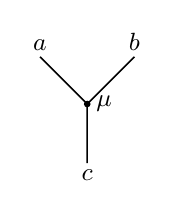
\begin{tikzpicture}[diagram]
  \draw (0,0.9) -- (0.6,0.3) (1.2,0.9) -- (0.6,0.3) -- (0.6,-0.45);
  \fvert{0.6,0.3}{\mu}
  \node[fleg, above] at (0,0.9) {$a$};
  \node[fleg, above] at (1.2,0.9) {$b$};
  \node[fleg, below] at (0.6,-0.45) {$c$};
\end{tikzpicture}

\smallskip
{\small The fusion vertex: the splitting intertwiner $\iota^{c\mu}_{ab}$ of
\eqref{eq:cgcdef}, read bottom to top, whose matrix elements are the CGC.}
\end{center}

\subsection{Orthonormality and completeness}

These are not conventions; they follow from Facts~\ref{fact:schur}
and~\ref{fact:pw}. Isometry of each $\iota^{c\mu}_{ab}$ and orthogonality of
distinct channels give
\begin{equation}\label{eq:ortho}
  \sum_{m_a,m_b}
    \overline{C^{c\mu}_{a\,m_a;\,b\,m_b}}\;
    C^{c'\mu'}_{a\,m_a;\,b\,m_b}
  \;=\; \delta_{cc'}\,\delta_{\mu\mu'}\,\delta_{m_c m_{c'}} ,
\end{equation}
and, since the channels together exhaust $V_a\otimes V_b$,
\begin{equation}\label{eq:complete}
  \sum_{c,\mu,m_c}
    C^{c\mu}_{a\,m_a;\,b\,m_b}\;
    \overline{C^{c\mu}_{a\,m_a';\,b\,m_b'}}
  \;=\; \delta_{m_a m_a'}\,\delta_{m_b m_b'} ,
\end{equation}
whose trace is the dimension count \eqref{eq:dimcount}. Equivalently: the
matrix $M[(m_a,m_b),(m_c,\mu)] = C^{c\mu}_{a m_a; b m_b}$ is unitary once the
column index runs over all $(c,\mu,m_c)$.

\code{racah} runs \eqref{eq:ortho} as a \emph{generation gate}: a residual
above tolerance is a typed error, never a silently returned coefficient.

\subsection{Gauge freedom}
\label{sec:gauge}

The CGC are not determined by $(a,b,c,\mu)$. Two choices are free:

\begin{enumerate}[label=(\alph*),leftmargin=2.0em]
  \item the orthonormal basis of each $V_x$, i.e. a unitary $U^x$ per irrep;
  \item when $N^c_{ab}>1$, how the $\mu$-copies are oriented inside the
    isotypic component, i.e. a unitary $V^{c}_{ab}\in U(N^c_{ab})$ mixing them.
\end{enumerate}

\begin{proposition}[The gauge group acting on CGC]\label{prop:gauge}
For unitaries $U^a,U^b,U^c$ and $V^c_{ab}\in U(N^c_{ab})$, the coefficients
\begin{equation}\label{eq:gaugetransform}
  \tilde C^{\,c\,\mu}_{a\,m_a;\,b\,m_b}
  \;=\; \sum_{\mu',\,n_a,\,n_b,\,n_c}
    V^{c}_{ab,\,\mu\mu'}\;
    U^{a}_{m_a n_a}\, U^{b}_{m_b n_b}\,
    \overline{U^{c}_{m_c n_c}}\;
    C^{\,c\,\mu'}_{a\,n_a;\,b\,n_b}
\end{equation}
satisfy \eqref{eq:cgcdef}--\eqref{eq:complete} for the transformed bases and
describe the same representation theory. This is the \emph{gauge freedom};
$\eqref{eq:gaugetransform}$ is the \emph{gauge transformation}. Note that (b)
is a genuinely per-$(a,b,c)$ freedom --- a unitary attached to each
multiplicity slot --- and is invisible whenever $N^c_{ab}\le 1$.
\end{proposition}

\begin{proposition}[What is gauge-invariant]
The orthogonal projector onto the $c$-isotypic component of $V_a\otimes V_b$,
\begin{equation}\label{eq:projector}
  \bigl[P^c_{ab}\bigr]_{(m_a,m_b),(m_a',m_b')}
  \;=\; \Bigl[\sum_{\mu}
    \iota^{c\mu}_{ab}\,\bigl(\iota^{c\mu}_{ab}\bigr)^\dagger\Bigr]
  \;=\; \sum_{\mu,\,m_c}
    C^{c\mu}_{a\,m_a;\,b\,m_b}\;
    \overline{C^{c\mu}_{a\,m_a';\,b\,m_b'}} ,
\end{equation}
is unchanged by \eqref{eq:gaugetransform} up to conjugation by
$U^a\otimes U^b$, and is completely invariant when the leg bases are held
fixed. It is therefore the right object for cross-implementation comparison.
\end{proposition}

\paragraph{Freezing a gauge.} ``Fixing the gauge'' means choosing, once and
deterministically, a representative of each gauge orbit --- as a specified
function of exact combinatorial data (the ordered basis, a pivot rule, a sign
rule, a descent order), never as ``whatever the current code happens to
output''. That distinction is the whole point of \gaugemd{} and \gaugeson{}:
under a frozen specification, a value contradicting a stated rule is a
\emph{bug} by definition, and a consumer's checkpointed coefficients stay valid
across refactors. \code{racah} freezes:

\begin{itemize}[leftmargin=1.4em]
  \item for $SU(N)$: the GT basis order, the coupling-pair column order, the
    nullspace tolerance and rank rule, the column-pivoted reduced-echelon pivot
    and tie-break, the positive-diagonal QR sign fix, and the reverse-lex
    descent order (\gaugemd{} \S1--\S8);
  \item for $B/C/D$: the Kronecker packing, the seed matrices, the QR gauge,
    the descending-weight sort and tie-break, the first-significant-entry block
    sign, the discovery-order multiplicity assignment, the canonical-parent
    rule, and the intertwiner alignment of rediscovered frames
    (\gaugeson{} \S1--\S16);
  \item for $SU(2)$: the closed-form phase/normalisation conventions
    (\gaugemd{} \S12).
\end{itemize}

Cross-checks against a \emph{different} convention necessarily go through the
gauge-invariant projector \eqref{eq:projector} or an explicit
gauge-transformation harness --- which is exactly how the QSpace CGC oracle for
$B/C/D$ is built $[3]$. Where the reference convention is the same, the check
is signed and element-wise: SUNRepresentations.jl $[9]$ for $SU(N)$, and the
\code{wigner-symbols} crate $[11]$ for $SU(2)$.

%======================================================================
\section{Recoupling: $6j$, $F$-symbols, $R$-symbols}
\label{sec:recoupling}
%======================================================================

Fusing three irreps $a,b,c$ into $d$ can be bracketed two ways, through an
intermediate $e$ on the left or $f$ on the right:
\[
  (V_a\otimes V_b)\otimes V_c \;\supset\; V_e\otimes V_c \;\supset\; V_d,
  \qquad
  V_a\otimes(V_b\otimes V_c) \;\supset\; V_a\otimes V_f \;\supset\; V_d .
\]
Both families of composites are bases of the same multiplicity space
$\Hom_G(V_d, V_a\otimes V_b\otimes V_c)$, so there is a unitary change of basis
between them. That unitary is the \emph{associator}, or $F$-symbol.

\subsection{$SU(2)$: the $6j$ symbol}

For $SU(2)$, where all multiplicities are $0$ or $1$, the change of basis is
Racah's $6j$ symbol
$\bigl\{\begin{smallmatrix} j_1 & j_2 & j_5 \\ j_3 & j_4 & j_6\end{smallmatrix}\bigr\}$,
which has a closed-form single-sum expression over products of factorials
$[5,16]$. It relates $(a\otimes b)\otimes c$ coupled through $e$ to
$a\otimes(b\otimes c)$ coupled through $f$, and \code{racah} evaluates it
exactly, keyed by its Regge symmetry class. The $F$-symbol is then obtained
from it by a fixed dimension-factor-and-phase dressing whose \emph{argument
order is itself gauge}; \gaugemd{} \S12 is the authority for that formula.
API: \code{wigner\_3j}, \code{wigner\_6j}, \code{su2\_f\_symbol},
\code{su2\_r\_symbol}.

\subsection{General $G$: the $F$-symbol as a four-CGC contraction}
\label{sec:fsymbol}

For general $G$ no closed form is available and $F$ is \emph{defined} by
contracting four CGC over every magnetic index, so that only the multiplicity
axes survive.

\begin{convention}[Axis order and vertex assignment of an $F$ block]
\label{conv:faxes}
A returned $F$ block is a dense rank-4 array
$[F^{abc}_d]_{e,f}[\mu,\nu,\kappa,\lambda]$, indexed by the two intermediate
labels $e,f$ and by four multiplicity indices, one per fusion vertex:
\[
  \underbrace{a\otimes b\to e}_{\displaystyle \mu\in[1,N^e_{ab}]},\quad
  \underbrace{e\otimes c\to d}_{\displaystyle \nu\in[1,N^d_{ec}]},\quad
  \underbrace{b\otimes c\to f}_{\displaystyle \kappa\in[1,N^f_{bc}]},\quad
  \underbrace{a\otimes f\to d}_{\displaystyle \lambda\in[1,N^d_{af}]}.
\]
So $e$ (with $\mu,\nu$) belongs to the \textbf{left} bracketing
$(a\otimes b)\otimes c$ and $f$ (with $\kappa,\lambda$) to the \textbf{right}
bracketing $a\otimes(b\otimes c)$; the axis lengths are
$[N^e_{ab},\,N^d_{ec},\,N^f_{bc},\,N^d_{af}]$ in that order, stored row-major,
matching the TensorKitSectors $[19]$ \code{GenericFusion} convention. The
contraction wiring and this axis order are shared between the $SU(N)$ and
$B/C/D$ engines by a single private core, so the convention cannot drift
between families. \gaugemd{} is the normative authority.
\end{convention}

With that assignment the definition \code{racah} implements is
\begin{equation}\label{eq:Fdef}
  \bigl[F^{abc}_{d}\bigr]_{e,f}[\mu,\nu,\kappa,\lambda]
  \;=\!\!\sum_{m_a,m_b,m_c,m_e,m_f}\!\!
    C^{\,e\,\mu}_{a\,m_a;\,b\,m_b}\;
    C^{\,d\,\nu}_{e\,m_e;\,c\,m_c}\Big|_{m_d}\;
    \overline{C^{\,f\,\kappa}_{b\,m_b;\,c\,m_c}}\;
    \overline{C^{\,d\,\lambda}_{a\,m_a;\,f\,m_f}\Big|_{m_d}} ,
\end{equation}
where the two CGC landing in $d$ are evaluated at one \emph{fixed} $d$-basis
index $m_d$ --- \code{racah} takes the first, $m_d=1$. Fixing rather than
summing is not an approximation: by Fact~\ref{fact:schur} the result is
independent of which $d$-state is used, which is itself a usable self-check.
If any of the four vertex multiplicities vanishes the block is empty; the
public wrappers report that as a typed \emph{zero fusion channel} error rather
than returning a zero block.

\begin{center}
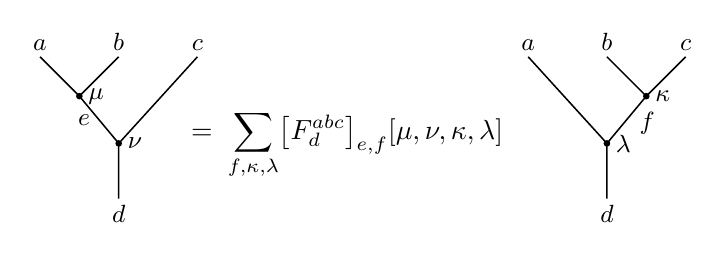
\begin{tikzpicture}[diagram, baseline={(0,0.4)}]
  % left-bracketed tree ((a b)_e c)_d
  \draw (0,1.6) -- (0.5,1.1) (1.0,1.6) -- (0.5,1.1)
        -- (1.0,0.5) (2.0,1.6) -- (1.0,0.5) -- (1.0,-0.2);
  \fvert{0.5,1.1}{\mu}\fvert{1.0,0.5}{\nu}
  \node[fleg, above] at (0,1.6) {$a$};
  \node[fleg, above] at (1.0,1.6) {$b$};
  \node[fleg, above] at (2.0,1.6) {$c$};
  \node[fleg, below] at (1.0,-0.2) {$d$};
  \node[fleg, left=1pt] at (0.75,0.8) {$e$};
  % equality and coefficient
  \node[anchor=base] at (3.9,0.55)
    {$=\;\displaystyle\sum_{f,\kappa,\lambda}
      \bigl[F^{abc}_{d}\bigr]_{e,f}[\mu,\nu,\kappa,\lambda]$};
  % right-bracketed tree (a (b c)_f)_d
  \begin{scope}[shift={(6.2,0)}]
    \draw (2.0,1.6) -- (1.5,1.1) (1.0,1.6) -- (1.5,1.1)
          -- (1.0,0.5) (0,1.6) -- (1.0,0.5) -- (1.0,-0.2);
    \fvert{1.5,1.1}{\kappa}\fvert{1.0,0.5}{\lambda}
    \node[fleg, above] at (0,1.6) {$a$};
    \node[fleg, above] at (1.0,1.6) {$b$};
    \node[fleg, above] at (2.0,1.6) {$c$};
    \node[fleg, below] at (1.0,-0.2) {$d$};
    \node[fleg, right=1pt] at (1.3,0.75) {$f$};
  \end{scope}
\end{tikzpicture}

\smallskip
{\small The $F$-move: the basis change computed by \eqref{eq:Fdef}, with the
four vertices labelled exactly as in Convention~\ref{conv:faxes}.}
\end{center}

\begin{remark}[Real CGC, elided conjugation]\label{rem:real}
In \code{racah}'s frozen gauge the CGC of \emph{every} family come out
real-valued: the $SU(N)$ construction solves a real nullspace and gauge-fixes
by a real echelon/QR pair, and the $B/C/D$ seeds are integer matrices carried
through real orthogonalisations. The implementation therefore elides the
conjugations in \eqref{eq:Fdef} and \eqref{eq:Rdef} --- value-identically, not
as an approximation. They are written here because they are part of the
definition, and because a future complex gauge would need them back.
\end{remark}

Unitarity of $F$ in the combined indices holds by
\eqref{eq:ortho}--\eqref{eq:complete}: arranging $F$ as a matrix $M$ with rows
$(e,\mu,\nu)$ and columns $(f,\kappa,\lambda)$,
\begin{equation}\label{eq:funitary}
  \sum_{f,\kappa,\lambda}
    \bigl[F^{abc}_d\bigr]_{e,f}[\mu,\nu,\kappa,\lambda]\;
    \overline{\bigl[F^{abc}_d\bigr]_{e',f}[\mu',\nu',\kappa,\lambda]}
  \;=\; \delta_{ee'}\delta_{\mu\mu'}\delta_{\nu\nu'} ,
\end{equation}
i.e. $M M^\dagger = \id$ ($M M^{\mathsf T} = \id$, $M$ being real). This is
shipped as a public self-check.

\subsection{The $R$-symbol}

The braiding exchanges the order of two fused irreps. Writing
$\tau_{ab}: V_a\otimes V_b \to V_b\otimes V_a$ for the flip $v\otimes w\mapsto
w\otimes v$, the composite $\tau_{ab}\circ\iota^{c\mu}_{ab}$ is an intertwiner
$V_c\to V_b\otimes V_a$, hence a combination of the $\iota^{c\nu}_{ba}$:
\begin{equation}\label{eq:Rdef}
  \tau_{ab}\circ \iota^{c\mu}_{ab}
  \;=\; \sum_{\nu} \bigl[R^{ab}_{c}\bigr]_{\mu\nu}\; \iota^{c\nu}_{ba},
  \qquad\text{i.e.}\qquad
  \bigl[R^{ab}_{c}\bigr]_{\mu\nu}
  \;=\; \sum_{m_a,m_b}
     C^{\,c\,\mu}_{a\,m_a;\,b\,m_b}\Big|_{m_c}\;
     \overline{C^{\,c\,\nu}_{b\,m_b;\,a\,m_a}\Big|_{m_c}} ,
\end{equation}
again at a single fixed $m_c$ (the first), for the same Schur-lemma reason as
in \eqref{eq:Fdef}. Note the index order in the second factor: its \emph{first}
magnetic slot is $m_b$, because it is a CGC of the coupling $b\otimes a\to c$.

\begin{center}
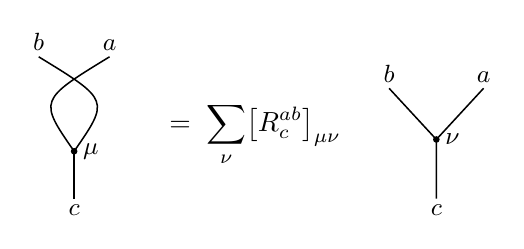
\begin{tikzpicture}[diagram, baseline={(0,0.35)}]
  % braided vertex: c splits via mu into a,b, then the flip crosses the legs
  \draw (0.6,0.2) .. controls (0.15,0.85) .. (1.05,1.4);
  \draw (0.6,0.2) .. controls (1.05,0.85) .. (0.15,1.4);
  \draw (0.6,0.2) -- (0.6,-0.4);
  \fvert{0.6,0.2}{\mu}
  \node[fleg, above] at (0.15,1.4) {$b$};
  \node[fleg, above] at (1.05,1.4) {$a$};
  \node[fleg, below] at (0.6,-0.4) {$c$};
  % equality and coefficient
  \node[anchor=base] at (2.9,0.45)
    {$=\;\displaystyle\sum_{\nu}\bigl[R^{ab}_{c}\bigr]_{\mu\nu}$};
  % plain vertex for b x a -> c
  \begin{scope}[shift={(4.6,0)}]
    \draw (0,1.0) -- (0.6,0.35) (1.2,1.0) -- (0.6,0.35) -- (0.6,-0.4);
    \fvert{0.6,0.35}{\nu}
    \node[fleg, above] at (0,1.0) {$b$};
    \node[fleg, above] at (1.2,1.0) {$a$};
    \node[fleg, below] at (0.6,-0.4) {$c$};
  \end{scope}
\end{tikzpicture}

\smallskip
{\small The $R$-move: the braiding
$\tau_{ab}\circ\iota^{c\mu}_{ab}=\sum_\nu[R^{ab}_c]_{\mu\nu}\,\iota^{c\nu}_{ba}$
of \eqref{eq:Rdef}.}
\end{center}

$R^{ab}_c$ is an $N^c_{ab}\times N^c_{ba}$ unitary --- \emph{not} square in
general, though $N^c_{ab}=N^c_{ba}$ always holds --- with rows indexed by $\mu$
and columns by $\nu$. In the multiplicity-free case it is a single phase, and
for $SU(2)$ it is $(-1)^{j_a+j_b-j_c}$ on an admissible triangle and exactly
$0$ otherwise (the zero mirrors $N^c_{ab}=0$ and stops a caller multiplying a
spurious sign into a forbidden channel). API:
\code{sun::\{f\_symbol, r\_symbol\}}, \code{bcd::\{f\_symbol, r\_symbol\}}.

\begin{remark}[No $6j$ outside $SU(2)$]
The recoupling surface for the generated families is $F$ and $R$ only. There is
no $6j$ function for $SU(N)$ or $B/C/D$: with outer multiplicity present the
$6j$'s scalar shape is not the natural object, and $F$ carries the same
information with the axes made explicit.
\end{remark}

%======================================================================
\section{The pentagon and hexagon identities}
\label{sec:pentagon}
%======================================================================

$F$ and $R$ are not free data. They are the associator and braiding of a
unitary braided fusion category, and as such must satisfy the coherence axioms
of Mac~Lane's theorem: the \emph{pentagon} (associativity of four-fold fusion)
and the two \emph{hexagons} (compatibility of braiding with fusion). The
axioms in the form used here are Etingof--Gelaki--Nikshych--Ostrik $[17]$
\S\S2.1, 8.1; the index-carrying physicist's form, with the same conventions
this crate follows, is Kitaev $[18]$ Appendix E.

Both are stated below in the \emph{exact index convention of the crate}: every
$F$ carries its four multiplicity axes in the order of
Convention~\ref{conv:faxes}, and $[F^{xyz}_{w}]_{u,v}[\cdot,\cdot,\cdot,\cdot]$
means the block for fusing $x,y,z$ into $w$ through $u$ (left) or $v$ (right).

\subsection{Pentagon}

Let $a,b,c,d$ be irreps and quantify over every
\[
  f\in a\otimes b,\quad h\in c\otimes d,\quad g\in f\otimes c,\quad
  i\in b\otimes h,\quad e\in (g\otimes d)\cap(a\otimes i).
\]
Then, for every value of the six \emph{free} multiplicity indices
\[
  \lambda\in[1,N^g_{fc}],\ \ \mu\in[1,N^e_{gd}],\ \ \nu\in[1,N^h_{cd}],\ \
  \kappa\in[1,N^f_{ab}],\ \ \rho\in[1,N^i_{bh}],\ \ \sigma\in[1,N^e_{ai}],
\]
the pentagon identity is
\begin{multline}\label{eq:pentagon}
  \sum_{\tau}\;
    \bigl[F^{fcd}_{e}\bigr]_{g,h}[\lambda,\mu,\nu,\tau]\;
    \bigl[F^{abh}_{e}\bigr]_{f,i}[\kappa,\tau,\rho,\sigma]
  \\[0.3em]
  \;=\;
  \sum_{j\,\in\, b\otimes c}\ \sum_{\alpha,\beta,\tau'}
    \bigl[F^{abc}_{g}\bigr]_{f,j}[\kappa,\lambda,\alpha,\beta]\;
    \bigl[F^{ajd}_{e}\bigr]_{g,i}[\beta,\mu,\tau',\sigma]\;
    \bigl[F^{bcd}_{i}\bigr]_{j,h}[\alpha,\tau',\nu,\rho] ,
\end{multline}
where the contracted multiplicity indices run over
$\tau\in[1,N^e_{fh}]$ on the left and, on the right,
$\alpha\in[1,N^j_{bc}]$, $\beta\in[1,N^g_{aj}]$, $\tau'\in[1,N^i_{jd}]$. A
label tuple for which any free-index range is empty is vacuous and skipped.
This is a condition on $F$ alone --- associativity of four-fold fusion.

\begin{center}
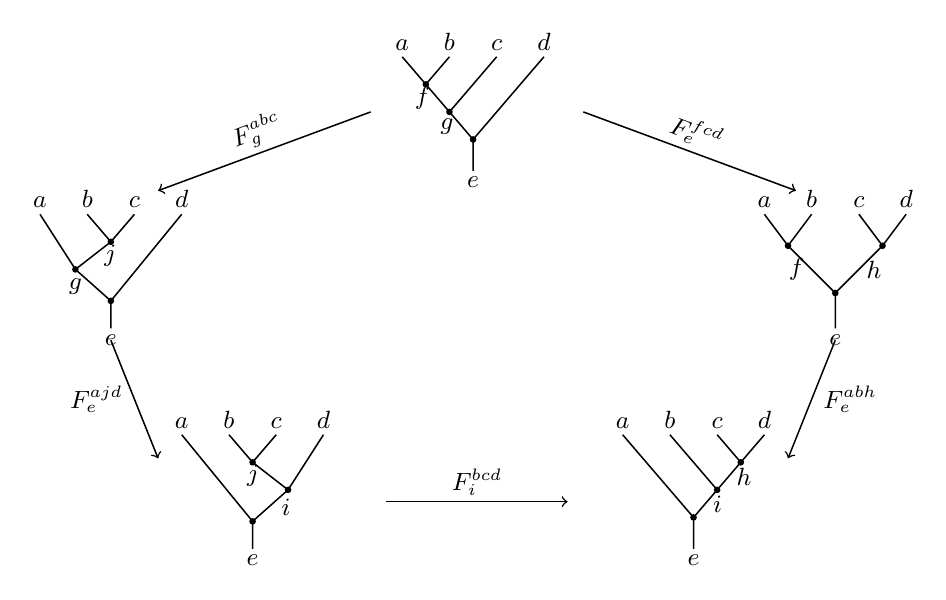
\begin{tikzpicture}[diagram]
  % T_A = ((ab)c)d, top centre
  \begin{scope}[shift={(4.6,4.4)}]
    \draw (0,1.2) -- (0.3,0.85) (0.6,1.2) -- (0.3,0.85) -- (0.6,0.5)
          (1.2,1.2) -- (0.6,0.5) -- (0.9,0.15) (1.8,1.2) -- (0.9,0.15)
          -- (0.9,-0.25);
    \node[fvertex] at (0.3,0.85) {};\node[fvertex] at (0.6,0.5) {};
    \node[fvertex] at (0.9,0.15) {};
    \node[fleg, above] at (0,1.2) {$a$};\node[fleg, above] at (0.6,1.2) {$b$};
    \node[fleg, above] at (1.2,1.2) {$c$};\node[fleg, above] at (1.8,1.2) {$d$};
    \node[fleg, left=0.5pt] at (0.45,0.67) {$f$};
    \node[fleg, left=0.5pt] at (0.75,0.32) {$g$};
    \node[fleg, below] at (0.9,-0.25) {$e$};
  \end{scope}
  % T_B = (ab)(cd), right upper
  \begin{scope}[shift={(9.2,2.4)}]
    \draw (0,1.2) -- (0.3,0.8) (0.6,1.2) -- (0.3,0.8) -- (0.9,0.2)
          (1.2,1.2) -- (1.5,0.8) (1.8,1.2) -- (1.5,0.8) -- (0.9,0.2)
          -- (0.9,-0.25);
    \node[fvertex] at (0.3,0.8) {};\node[fvertex] at (1.5,0.8) {};
    \node[fvertex] at (0.9,0.2) {};
    \node[fleg, above] at (0,1.2) {$a$};\node[fleg, above] at (0.6,1.2) {$b$};
    \node[fleg, above] at (1.2,1.2) {$c$};\node[fleg, above] at (1.8,1.2) {$d$};
    \node[fleg, left=0.5pt] at (0.6,0.5) {$f$};
    \node[fleg, right=0.5pt] at (1.2,0.5) {$h$};
    \node[fleg, below] at (0.9,-0.25) {$e$};
  \end{scope}
  % T_C = a(b(cd)), right lower
  \begin{scope}[shift={(7.4,-0.4)}]
    \draw (1.2,1.2) -- (1.5,0.85) (1.8,1.2) -- (1.5,0.85) -- (1.2,0.5)
          (0.6,1.2) -- (1.2,0.5) -- (0.9,0.15) (0,1.2) -- (0.9,0.15)
          -- (0.9,-0.25);
    \node[fvertex] at (1.5,0.85) {};\node[fvertex] at (1.2,0.5) {};
    \node[fvertex] at (0.9,0.15) {};
    \node[fleg, above] at (0,1.2) {$a$};\node[fleg, above] at (0.6,1.2) {$b$};
    \node[fleg, above] at (1.2,1.2) {$c$};\node[fleg, above] at (1.8,1.2) {$d$};
    \node[fleg, right=0.5pt] at (1.35,0.67) {$h$};
    \node[fleg, right=0.5pt] at (1.05,0.32) {$i$};
    \node[fleg, below] at (0.9,-0.25) {$e$};
  \end{scope}
  % T_D = (a(bc))d, left upper
  \begin{scope}[shift={(0,2.4)}]
    \draw (0.6,1.2) -- (0.9,0.85) (1.2,1.2) -- (0.9,0.85) -- (0.45,0.5)
          (0,1.2) -- (0.45,0.5) -- (0.9,0.1) (1.8,1.2) -- (0.9,0.1)
          -- (0.9,-0.25);
    \node[fvertex] at (0.9,0.85) {};\node[fvertex] at (0.45,0.5) {};
    \node[fvertex] at (0.9,0.1) {};
    \node[fleg, above] at (0,1.2) {$a$};\node[fleg, above] at (0.6,1.2) {$b$};
    \node[fleg, above] at (1.2,1.2) {$c$};\node[fleg, above] at (1.8,1.2) {$d$};
    \node[fleg, right=0.5pt] at (0.72,0.68) {$j$};
    \node[fleg, left=0.5pt] at (0.63,0.28) {$g$};
    \node[fleg, below] at (0.9,-0.25) {$e$};
  \end{scope}
  % T_E = a((bc)d), left lower
  \begin{scope}[shift={(1.8,-0.4)}]
    \draw (0.6,1.2) -- (0.9,0.85) (1.2,1.2) -- (0.9,0.85) -- (1.35,0.5)
          (1.8,1.2) -- (1.35,0.5) -- (0.9,0.1) (0,1.2) -- (0.9,0.1)
          -- (0.9,-0.25);
    \node[fvertex] at (0.9,0.85) {};\node[fvertex] at (1.35,0.5) {};
    \node[fvertex] at (0.9,0.1) {};
    \node[fleg, above] at (0,1.2) {$a$};\node[fleg, above] at (0.6,1.2) {$b$};
    \node[fleg, above] at (1.2,1.2) {$c$};\node[fleg, above] at (1.8,1.2) {$d$};
    \node[fleg, left=0.5pt] at (1.08,0.68) {$j$};
    \node[fleg, right=0.5pt] at (1.17,0.28) {$i$};
    \node[fleg, below] at (0.9,-0.25) {$e$};
  \end{scope}
  % the five F-moves
  \draw[->] (6.9,4.9) -- (9.6,3.9)
    node[fleg, midway, above, sloped] {$F^{fcd}_{e}$};
  \draw[->] (10.1,2.0) -- (9.5,0.5)
    node[fleg, midway, right=2pt] {$F^{abh}_{e}$};
  \draw[->] (4.2,4.9) -- (1.5,3.9)
    node[fleg, midway, above, sloped] {$F^{abc}_{g}$};
  \draw[->] (0.9,2.0) -- (1.5,0.5)
    node[fleg, midway, left=2pt] {$F^{ajd}_{e}$};
  \draw[->] (4.4,-0.05) -- (6.7,-0.05)
    node[fleg, midway, above] {$F^{bcd}_{i}$};
\end{tikzpicture}

\smallskip
{\small The pentagon \eqref{eq:pentagon}: the two-move route (right side, the
left-hand side of the equation) and the three-move route (left side) between
the same two bracketings agree; multiplicity labels as in \eqref{eq:pentagon}.}
\end{center}

\subsection{Hexagons}

Quantify over every
$e\in c\otimes a$, $f\in c\otimes b$, $d\in (e\otimes b)\cap(a\otimes f)$, and
every value of the free indices
\[
  \alpha\in[1,N^e_{ca}],\quad \beta\in[1,N^d_{eb}],\quad
  \mu\in[1,N^f_{bc}],\quad \nu\in[1,N^d_{af}].
\]
The first hexagon is
\begin{multline}\label{eq:hexagon}
  \sum_{\lambda,\gamma}\;
    \bigl[R^{ca}_{e}\bigr]_{\alpha\lambda}\;
    \bigl[F^{acb}_{d}\bigr]_{e,f}[\lambda,\beta,\gamma,\nu]\;
    \bigl[R^{cb}_{f}\bigr]_{\gamma\mu}
  \\[0.3em]
  \;=\;
  \sum_{g\,\in\, a\otimes b}\ \sum_{\delta,\sigma,\psi}
    \bigl[F^{cab}_{d}\bigr]_{e,g}[\alpha,\beta,\delta,\sigma]\;
    \bigl[R^{cg}_{d}\bigr]_{\sigma\psi}\;
    \bigl[F^{abc}_{d}\bigr]_{g,f}[\delta,\psi,\mu,\nu] ,
\end{multline}
with contracted indices $\lambda\in[1,N^e_{ac}]$, $\gamma\in[1,N^f_{cb}]$ on
the left and $\delta\in[1,N^g_{ab}]$, $\sigma\in[1,N^d_{cg}]$,
$\psi\in[1,N^d_{gc}]$ on the right. The second hexagon is
\eqref{eq:hexagon} with the three braidings replaced by the opposite ones and
conjugated,
\[
  R^{ca}_e \rightsquigarrow \overline{R^{ac}_e},\qquad
  R^{cb}_f \rightsquigarrow \overline{R^{bc}_f},\qquad
  R^{cg}_d \rightsquigarrow \overline{R^{gc}_d},
\]
which is the $R\mapsto R^{-1}$ form of the axiom written out; since $R$ is real
in this gauge (Remark~\ref{rem:real}) the conjugations are elided in the
implementation and the two hexagons differ only in the argument order of the
three $R$ blocks.

\begin{remark}[Status in the implementation]
\eqref{eq:pentagon} and \eqref{eq:hexagon} are shipped as \emph{public
self-checks} and additionally run as \emph{generation gates}: a violation
beyond tolerance is a typed error, never a silently returned coefficient. They
are the strongest available consistency statement about numerically constructed
CGC, because they constrain the whole coefficient set jointly rather than one
block at a time. The equations, index conventions and the generic-multiplicity
branch follow TensorKitSectors $[19]$; see \refsmd{} for the
\code{file:symbol}-level rows.
\end{remark}

\begin{remark}[Gauge covariance of the axioms]
A gauge transformation \eqref{eq:gaugetransform} changes $F$ and $R$ but
preserves \eqref{eq:pentagon} and \eqref{eq:hexagon}: the transformation acts
on $F$ by conjugation with the $V$'s on each of the four multiplicity slots and
the $U$'s cancel. So passing the pentagon and hexagon certifies
\emph{consistency}, not agreement with any particular convention. Convention
agreement is a separate claim, and it is settled by the oracles of
Section~\ref{sec:exact} against the pinned reference implementations.
\end{remark}

%======================================================================
\section{What is exact, and what is verification-gated}
\label{sec:exact}
%======================================================================

The note's objects split cleanly into combinatorial data and solved data, and
the implementation's contract follows that split.

\paragraph{Exact / combinatorial.} Irrep labels and dominance; the Weyl
dimension \eqref{eq:weyldim}; duals; Frobenius--Schur indicators
\eqref{eq:fs}; fusion multiplicities \eqref{eq:fusion}; weight systems
\eqref{eq:freudenthal}; GT pattern enumeration and basis ordering; and, for
$SU(2)$ only, the full $3j$/$6j$/CGC/$F$/$R$ values, carried as signed
square-rooted rationals with a single final rounding.

\paragraph{Numeric / verification-gated.} For the generated families the CGC
--- and the $F$, $R$ contracted from them by \eqref{eq:Fdef},
\eqref{eq:Rdef} --- come from a nullspace solve and are floating point. Their
\emph{values} are finite precision, but the \emph{gauge} fixing them is a
deterministic function of exact combinatorial data, and every generation runs
the orthonormality \eqref{eq:ortho}, unitarity \eqref{eq:funitary}, pentagon
\eqref{eq:pentagon} and hexagon \eqref{eq:hexagon} checks before returning.

So ``exact'' in this project is a claim about \textbf{structure, gauge
determinism, and verification}, not about symbolic algebraic-number
coefficient values.

\paragraph{Independent oracles.} Consistency checks cannot detect a systematic
convention divergence (see the gauge-covariance remark in
Section~\ref{sec:pentagon}), so each family is additionally checked against an
implementation that is not this one:

\begin{center}
\small
\begin{tabular}{@{}lll@{}}
\toprule
Family & Oracle & Nature of the comparison \\
\midrule
$SU(2)$ & \code{wigner-symbols} crate v0.5.1 $[11]$ & exhaustive over its label domain \\
$SU(N)$ & SUNRepresentations.jl v0.4.0 $[9]$ & signed, element-wise, including the $\mu$ order \\
$SU(N)$ & GroupMath v1.1.3 $[6]$ & products and multiplicities \\
$SO(N)$, $Sp(2N)$ & QSpace v4 $[3]$ & projector battery \eqref{eq:projector} \\
$B/C/D$ dims & QSpace v4 $[3]$ & exact dimension agreement \\
\bottomrule
\end{tabular}
\end{center}

The $SU(2)$ and $SU(N)$ comparisons are signed and element-wise because
\code{racah} adopts those references' conventions outright; the $B/C/D$
comparison goes through the gauge-invariant projector
\eqref{eq:projector} because \code{racah}'s $B/C/D$ gauge deliberately deviates
from QSpace's in documented, enumerated ways (\gaugeson{}).

%======================================================================
\begin{thebibliography}{21}

\bibitem{alex} A. Alex, M. Kalus, A. Huckleberry, J. von Delft,
``A numerical algorithm for the explicit calculation of $SU(N)$ and
$SL(N,\CC)$ Clebsch--Gordan coefficients,''
\emph{J. Math. Phys.} \textbf{52}, 023507 (2011).
\href{https://doi.org/10.1063/1.3521562}{doi:10.1063/1.3521562};
\href{https://arxiv.org/abs/1009.0437}{arXiv:1009.0437}.

\bibitem{weichselbaum2012} A. Weichselbaum,
``Non-abelian symmetries in tensor networks: A quantum symmetry space
approach,'' \emph{Ann. Phys.} \textbf{327}, 2972--3047 (2012).
\href{https://doi.org/10.1016/j.aop.2012.07.009}{doi:10.1016/j.aop.2012.07.009};
\href{https://arxiv.org/abs/1202.5664}{arXiv:1202.5664}.

\bibitem{qspace} A. Weichselbaum,
``QSpace --- An open-source tensor library for Abelian and non-Abelian
symmetries,'' \emph{SciPost Phys. Codebases} \textbf{40} (2024).
\href{https://doi.org/10.21468/SciPostPhysCodeb.40}{doi:10.21468/SciPostPhysCodeb.40};
\href{https://arxiv.org/abs/2405.06632}{arXiv:2405.06632}.
\code{racah} cites QSpace v4 source at revision \code{dd2cc7e}.

\bibitem{gt1950} I. M. Gelfand, M. L. Tsetlin,
``Finite-dimensional representations of the group of unimodular matrices,''
\emph{Dokl. Akad. Nauk SSSR} \textbf{71}, 825--828 (1950) (Russian).
No DOI (predates DOI registration).

\bibitem{racah1942} G. Racah, ``Theory of Complex Spectra. II,''
\emph{Phys. Rev.} \textbf{62}, 438--462 (1942).
\href{https://doi.org/10.1103/PhysRev.62.438}{doi:10.1103/PhysRev.62.438}.

\bibitem{groupmath} R. M. Fonseca,
``GroupMath: A Mathematica package for group theory calculations,''
\emph{Comput. Phys. Commun.} \textbf{267}, 108085 (2021).
\href{https://doi.org/10.1016/j.cpc.2021.108085}{doi:10.1016/j.cpc.2021.108085};
\href{https://arxiv.org/abs/2011.01764}{arXiv:2011.01764}.
\code{racah} fixtures use GroupMath v1.1.3.

\bibitem{fultonharris} W. Fulton, J. Harris,
\emph{Representation Theory: A First Course},
Graduate Texts in Mathematics \textbf{129}, Springer (1991).
ISBN 0-387-97495-4.
\href{https://doi.org/10.1007/978-1-4612-0979-9}{doi:10.1007/978-1-4612-0979-9}.

\bibitem{humphreys} J. E. Humphreys,
\emph{Introduction to Lie Algebras and Representation Theory},
Graduate Texts in Mathematics \textbf{9}, Springer (1972).
ISBN 978-0-387-90053-7.
\href{https://doi.org/10.1007/978-1-4612-6398-2}{doi:10.1007/978-1-4612-6398-2}.

\bibitem{sunreps} SUNRepresentations.jl (v0.4.0), a Julia implementation of
$[1]$. \url{https://github.com/QuantumKitHub/SUNRepresentations.jl}.

\bibitem{wignersymbolsjl} WignerSymbols.jl (v2.0.0), J. Haegeman.
\url{https://github.com/Jutho/WignerSymbols.jl}.

\bibitem{wignersymbolsrs} \code{wigner-symbols} Rust crate (v0.5.1),
P. Ruffwind. \url{https://crates.io/crates/wigner-symbols}.

\bibitem{molev} A. I. Molev, ``Gelfand--Tsetlin bases for classical Lie
algebras,'' in \emph{Handbook of Algebra} \textbf{4}, M. Hazewinkel (ed.),
Elsevier (2006), pp. 109--170.
\href{https://doi.org/10.1016/S1570-7954(06)80006-9}{doi:10.1016/S1570-7954(06)80006-9};
\href{https://arxiv.org/abs/math/0211289}{arXiv:math/0211289}.

\bibitem{slansky} R. Slansky, ``Group theory for unified model building,''
\emph{Phys. Rep.} \textbf{79}, 1--128 (1981).
\href{https://doi.org/10.1016/0370-1573(81)90092-2}{doi:10.1016/0370-1573(81)90092-2}.
Congruency classes: \S5, p.~37; table notes for Table~36 ($SO(8)$) and
Table~41 ($SO(10)$).

\bibitem{brockertomdieck} T. Br\"ocker, T. tom Dieck,
\emph{Representations of Compact Lie Groups},
Graduate Texts in Mathematics \textbf{98}, Springer (1985).
ISBN 978-3-540-13678-1.
\href{https://doi.org/10.1007/978-3-662-12918-0}{doi:10.1007/978-3-662-12918-0}.
\emph{Added for this note:} Haar averaging and complete reducibility
(\S II.1--II.4), Peter--Weyl and Schur orthogonality (\S III.3), and the
Frobenius--Schur indicator (\S II.6).

\bibitem{bairdbiedenharn} G. E. Baird, L. C. Biedenharn,
``On the Representations of the Semisimple Lie Groups. II,''
\emph{J. Math. Phys.} \textbf{4}, 1449--1466 (1963).
\href{https://doi.org/10.1063/1.1703926}{doi:10.1063/1.1703926}.
\emph{Added for this note:} the explicit closed-form matrix elements of the
$\g\mathfrak{l}_N$ generators in the Gelfand--Tsetlin basis, which
Fact~\ref{fact:gt} states and the $SU(N)$ construction consumes.

\bibitem{wigner1959} E. P. Wigner,
\emph{Group Theory and its Application to the Quantum Mechanics of Atomic
Spectra}, Academic Press (1959).
\emph{Added for this note:} the Wigner--Eckart framework and the $3j$ symmetry
structure underlying the $SU(2)$ closed forms.

\bibitem{egno} P. Etingof, S. Gelaki, D. Nikshych, V. Ostrik,
\emph{Tensor Categories}, Mathematical Surveys and Monographs \textbf{205},
American Mathematical Society (2015). ISBN 978-1-4704-2024-6.
\href{https://doi.org/10.1090/surv/205}{doi:10.1090/surv/205}.
\emph{Added for this note:} the fusion-category axioms --- pentagon (\S2.1) and
hexagon (\S8.1) --- as the source for
\eqref{eq:pentagon} and \eqref{eq:hexagon}.

\bibitem{kitaev} A. Kitaev, ``Anyons in an exactly solved model and beyond,''
\emph{Ann. Phys.} \textbf{321}, 2--111 (2006).
\href{https://doi.org/10.1016/j.aop.2005.10.005}{doi:10.1016/j.aop.2005.10.005};
\href{https://arxiv.org/abs/cond-mat/0506438}{arXiv:cond-mat/0506438}.
\emph{Added for this note:} Appendix E, the index-carrying ($F$, $R$,
Frobenius--Schur) conventions in the form this crate's conventions follow.

\bibitem{tks} TensorKitSectors.jl, the categorical-symmetry layer of TensorKit.
\url{https://github.com/QuantumKitHub/TensorKitSectors.jl}.
\emph{Added for this note as a numbered entry} (\refsmd{} cites it inline at
\code{file:symbol} level): the pinned source for the $F$/$R$ contraction wiring
and axis order (\code{sectors.jl:Fsymbol\_from\_fusiontensor}), the
pentagon/hexagon index conventions
(\code{sectors.jl:pentagon\_equation}, \code{hexagon\_equation}), and the
$SU(2)$ $F$/$R$/Frobenius--Schur conventions
(\code{irreps/su2irrep.jl}). It is the \textbf{pinned convention oracle} for
$SU(2)$: where the mathematics admits several conventions, \code{racah}'s
choice is by definition TensorKitSectors' choice.

\bibitem{bourbaki} N. Bourbaki, \emph{Lie Groups and Lie Algebras,
Chapters 4--6}, Elements of Mathematics, Springer (2002).
ISBN 978-3-540-42650-9.
\href{https://doi.org/10.1007/978-3-540-89394-3}{doi:10.1007/978-3-540-89394-3}.
\emph{Added for this note:} the simple-root numbering (Plates I--IX) that fixes
the order of the Dynkin label tuple in the API; Ch.~VI \S4 (Theorem~3 and the
plates) for the Killing--Cartan classification, the nine Dynkin diagrams, the
low-rank identifications (\S4.4), and the tabulated $P/Q$ of each family.

\bibitem{knapp} A. W. Knapp, \emph{Lie Groups Beyond an Introduction},
2nd ed., Progress in Mathematics \textbf{140}, Birkh\"auser (2002).
ISBN 978-0-8176-4259-4.
\href{https://doi.org/10.1007/978-1-4757-2453-0}{doi:10.1007/978-1-4757-2453-0}.
\emph{Added for this note:} existence of a compact real form of a complex
semisimple Lie algebra (Theorem~6.11) and its uniqueness up to conjugacy
(Corollary~6.20) --- the step from the classification of algebras to the
compact groups \code{racah} computes for.

\end{thebibliography}

\end{document}
